
\PassOptionsToPackage{prologue,dvipsnames}{xcolor}
\documentclass{article}
\usepackage{fullpage}
\usepackage{microtype}
\usepackage{graphicx}
\usepackage{subcaption}
\usepackage{multirow}
\usepackage{placeins}
\usepackage{booktabs, colortbl} 
\usepackage{natbib}
\usepackage[colorlinks=true, linkcolor=BrickRed, citecolor=darkgreen, urlcolor=blue]{hyperref}




\let\oldemph\emph
\renewcommand{\emph}[1]{{\color{BrickRed}\oldemph{#1}}}


\newcommand{\theHalgorithm}{\arabic{algorithm}}
\usepackage{wrapfig}


\usepackage{amsmath}
\usepackage{amssymb}
\usepackage{mathtools}
\usepackage{amsthm}


\usepackage[capitalize,noabbrev,nameinlink]{cleveref}


\theoremstyle{definition}
\newtheorem{theorem}{Theorem}
\newtheorem{proposition}[theorem]{Proposition}
\newtheorem{lemma}[theorem]{Lemma}
\newtheorem{corollary}[theorem]{Corollary}

\newtheorem{definition}{Definition}
\newtheorem{assumption}{Assumption}
\theoremstyle{remark}
\newtheorem{remark}[theorem]{Remark}


\usepackage[textsize=tiny]{todonotes}


\usepackage{booktabs}       
\usepackage{nicefrac}       
\usepackage{microtype}      
\usepackage{xcolor}         
\usepackage{xspace}



\usepackage[T1]{fontenc}

\usepackage{tikz}
\usetikzlibrary{patterns}
\usetikzlibrary{calc}
\usetikzlibrary{arrows.meta}
\usetikzlibrary{positioning}
\usetikzlibrary{shapes.geometric}
\usetikzlibrary{decorations.pathreplacing}
\usepackage{pgfplots}
\pgfplotsset{compat=1.18}


\usepackage{amsmath}
\DeclareMathOperator{\alg}{ALG}
\DeclareMathOperator{\opt}{OPT}
\DeclareMathOperator{\prm}{\mathsf{PR}}
\DeclareMathOperator{\katz}{\mathsf{K}}
\DeclareMathOperator*{\argmax}{arg\,max}
\DeclareMathOperator*{\argmin}{arg\,min}
\usepackage{mathtools}
\DeclarePairedDelimiter\ceil{\lceil}{\rceil}
\DeclarePairedDelimiter\floor{\lfloor}{\rfloor}
\newcommand{\np}{{\textup{NP}}}


\newcommand{\absorbrank}{{\textsc{AbsorbRank}}\xspace}
\newcommand{\absorbkatz}{{\textsc{AbsorbKatz}}\xspace}
\newcommand{\mesrank}{{\textsc{MesRank}}\xspace}
\newcommand{\meskatz}{{\textsc{MesKatz}}\xspace}
\newcommand{\bosrank}{{\textsc{BosRank}}\xspace}
\newcommand{\boskatz}{{\textsc{BosKatz}}\xspace}
\newcommand{\seqabsorbrank}{{\textsc{SeqAbsorbRank}}\xspace}
\newcommand{\seqabsorb}{{\textsc{SeqAbsorb}}\xspace}
\newcommand{\seqabsorbkatz}{{\textsc{SeqAbsorbKatz}}\xspace}
\newcommand{\toprank}{{\textsc{TopRank}}\xspace}
\newcommand{\topkatz}{{\textsc{TopKatz}}\xspace}
\renewcommand{\top}{{\textsc{Top}}\xspace}
\usepackage[T1]{fontenc}
\newcommand{\Was}{Wa\k{\ \!}\hspace{-0.025cm}s}
\newcommand{\Succ}{S\!ucc}
\newcommand{\Pred}{Pred}

\newcommand{\appendixstart}{\color{gray}\textbf{Appendix:}}
\newcommand{\appendixend}{\color{black}}


\usepackage{txfonts}

\usepackage{pifont}
\definecolor{crimson}{RGB}{220, 20, 60}
\definecolor{darkgreen}{rgb}{0,0.5,0}
\newcommand{\no}{\textcolor{BrickRed}{\ding{55}}}
\newcommand{\yes}{\textcolor{darkgreen}{\ding{51}}}
\definecolor{mossgreen}{rgb}{0.68, 0.87, 0.68}


\usepackage{amsthm}
\newtheorem{example}{Example}
\newtheorem{claim}{Claim}
\newtheorem{observation}{Observation}

\usepackage{cleveref}



  \tikzset{     
    e4c node/.style={circle,draw,minimum size=0.3cm,inner sep=0,font=\tiny},
    e4b node/.style={circle,draw,minimum size=0.8cm,inner sep=0,font=\normalsize},
    selected/.style={draw=BrickRed,double}, 
    selected2/.style={preaction={fill, OliveGreen!45}}, 
    selected3/.style={pattern=north east lines, pattern color=NavyBlue}, 
    e4c edge/.style={sloped,above,font=\footnotesize,-{Classical TikZ Rightarrow[length=0.75mm]},draw,thin},
    e4c path/.style={-{Classical TikZ Rightarrow[length=0.75mm]},draw,thin}
  }


\makeatletter
\renewenvironment{description}%
               {\list{}{%
                   \setlength{\labelwidth}{\z@}%
                   \setlength{\labelsep}{1pt}% Adjust label separation
                   \setlength{\leftmargin}{0pt}% Adjust left margin
                   \setlength{\itemsep}{2pt}%% Decrease space between items
                   \setlength{\parsep}{2pt}%% Decrease space between paragraphs
                   \setlength{\topsep}{2pt}%% Reduce space before the environment
                   \setlength{\parskip}{2pt}%% Reduce space before the environment
                   \setlength{\itemindent}{\z@}%
                   \let\makelabel\descriptionlabel}}%
               {\endlist}
\makeatother

\title{Proportional Selection in Networks}

\usepackage{authblk}
\renewcommand{\Authfont}{\large}

\date{}

\author[1]{Georgios Papasotiropoulos}
\author[1]{Oskar Skibski}
\author[1]{Piotr Skowron}
\author[2]{Tomasz \Was}

\affil[1]{{\small{University of Warsaw}}}
\affil[2]{{\small{University of Oxford}}}

\begin{document}






\vskip 0.3in



\maketitle
\begin{abstract}
We address the problem of selecting $k$ representative nodes from a network, aiming to achieve two objectives: identifying the most influential nodes and ensuring the selection proportionally reflects the network's diversity. We propose two approaches to accomplish this, analyze them theoretically, and demonstrate their effectiveness through a series of experiments.
\end{abstract}

\section{Introduction}

Consider the problem of selecting a fixed number of $k$ nodes from a network. Our goal is twofold: to identify the most influential nodes, and to ensure that the selection proportionally represents the diversity within the network. 
For instance, consider a network composed of three groups of densely connected nodes. Assume the groups contain 50\%, 30\%, and 20\% of all nodes, respectively, and connections between groups are relatively sparse. If the objective is to select $k = 10$ nodes, a proportional approach would involve selecting five most influential nodes from the first group, three from the second, and two from the third group. In this paper we design selection methods that capture this intuition, yet apply to networks with more complex structures.

Our model has broad applicability across various real-world scenarios. For instance, imagine a network where nodes represent political blogs or news websites, and the links indicate references between them. In this context, proportional selection would ensure a balanced representation of predominant opinions, such as left-wing and right-wing political views, within the chosen set of websites. As another example consider the case of a strike group described by~\citet{Michael:1997}: After acquiring a forest products facility, new management revised workers' compensation, prompting a strike. When negotiations stalled, external consultants analyzed the workers' communication network, revealing three distinct groups: young Spanish speakers, young English speakers, and older English speakers. Consultants identified Bob and Norm as key communicators and, by engaging them, quickly resolved the strike. Interestingly, for $k=2$, our methods identify the same individuals. When $k=3$, our best-performing method also selects Alejandro, ensuring representation from each of the predominant groups.

Finally, our model generalizes elections. As discussed in \Cref{sec:case-studies}, for bipartite graphs, it reduces to a well-studied election framework where proportionality is extensively explored~\citep{lac-sko:b:approval-survey, FSST-trends}. From what follows our work contributes to the social choice literature by enabling elections where the set of candidates is not predetermined. Instead, citizens can cast their votes for individuals they know personally. This concept has been previously explored in the context of vote delegation, or liquid democracy~\citep{green2015direct, brill2018interactive}. However, liquid democracy often faces criticism because delegated votes tend to concentrate in the hands of a single influential individual. In contrast, our approach focuses on selecting a group of representatives based on votes cast through personal connections and trust. Thus, our approach combines the benefits of indirect democracy with a more personalized voting process, fostering a stronger connection between voters and their representatives.

Numerous measures of node importance has been proposed,
and they are commonly known as centralities.
In this paper, we propose two approaches that define selection rules for representative nodes
based on given centrality measures. 
While our approaches are general and compatible with most prominent centrality measures as well as machine learning models,
we focus here on two particular examples: PageRank~\citep{PagBriMotWin-1999-PageRank} and Katz centrality~\citep{Kat-1953-KatzCentrality}. Our first approach constructs elections from the underlying graphs and applies contemporary methods from social choice theory. 
In the second approach, we evaluate subsets of nodes by modifying the original graph; specifically we prevent selected nodes from propagating their accumulated influence, hence limiting the extent to which a well-represented part of the network influences the assesment of remaining nodes. 
We analyze our methods axiomatically and characterize their behavior on special graph classes, where proportional selection is intuitively demonstrated. Our extensive experiments prove the potential for applying our methods in real scenarios.

Our work relates to research on group centrality measures~\citep{everett1999centrality,angriman2020group} and the strategic aspects of nodes selection in networks~\citep{alon2011sum,holzman2013impartial,aziz2016strategyproof}, yet, to the best of our knowledge, the notion of proportional representation has not been explored in either context.
It also aligns with studies on proportional clustering \citep{AziLeeChuVol-2023-PropCentroids,CheFaiLyuMun-2019-PropClustering,LiLiSunWanWan-2021-PropClustering}, which focus on distance-based division of the nodes into groups rather than on selecting nodes based on their influence. 

\medskip
All proofs can be found in the Appendix.

\section{Preliminaries}
\label{sec:prelims}
We consider unweighted simple directed graphs.
We will interpret nodes as voters and outgoing edges as their support for other nodes, or simply their votes.
A \emph{graph} (or a \emph{network}) is a pair, $G = (V,E)$, where $V$ is a set of $n$ nodes and $E \subseteq V \times V$ is a set of $m$ edges; the edges are ordered pairs of nodes.
An edge $(u,v)$ is an \emph{outgoing edge} for node $u$ and an \emph{incoming edge} for $v$.
The set of outgoing edges of $u$ is denoted by $E^+(u)$.
For a set of nodes $S \subseteq V$, we let $E^+(S) = \bigcup_{u \in S} E^+(u)$.
The number of outgoing (resp. incoming) edges of $u$ is called \emph{out-degree} (resp. \emph{in-degree}) of $u$ and denoted by $\deg^+(u)$ (resp. $\deg^-(u)$).

A \emph{walk} is a sequence of nodes $(v_1,\dots,v_k)$ such that every two consecutive nodes are connected by an edge: $(v_i,v_{i+1}) \in E$ for every $i \in {1,\dots,k-1}$.
The length of such a walk is equal to $k-1$, i.e., the number of edges in the walk.
Note that a single node is a walk of length 0.
If in a walk all nodes are distinct, we call it a \emph{path}.
A node $u$ is called a \emph{predecessor} of $w$ if there exists a walk $(v_1,\dots,v_k)$ such that $u = v_1$ and $w = v_k$.
A node $u$ is a \emph{successor} of $w$ if $w$ is a predecessor of $u$.
The set of predecessors of node $u$ is denoted by $Pred(u)$ and its set of successors is denoted by $\Succ(u)$.
For a set of nodes $S \subseteq V$ we define 
% $Pred(S) = \bigcup_{u \in S} Pred(u)$ and 
$\Succ(S) = \bigcup_{u \in S} \Succ(u)$.
The set of all walks in $G$ is denoted by $\Omega(G)$.

For a set of nodes $S \subseteq V$, we denote by $G[S]$ the graph $(S,\{(u,v) \in E: u,v \in S\})$, i.e., the graph containing $S$ and the edges between nodes from $S$\!.
For a set of edges $M \subseteq E$, we denote by $G-M$ the graph $(V,E\setminus M),$ i.e., the subgraph of $G$ that remains after the deletion of edges in $M$.
A \emph{(weakly connected) component} of $G$ is a (maximal) subset of nodes $S \subseteq V$ such that every two nodes are connected by a walk in the \emph{underlying} (undirected) graph inferred by $G$.
A (sub)graph $G$ is \emph{strongly connected} if for every two nodes $u,v$ of $G$ there exists a walk from $u$ to $v$.
In particular, a \emph{strongly connected component} is a component which is strongly connected. A \emph{clique} is a graph in which every two nodes $u,v$ are connected by an edge.

A graph $G=(V,E)$ is called (directed) \emph{bipartite} if all walks in $\Omega(G)$ are of length of at most $1$, in other words, if its set of nodes $V$ can be divided into two disjoint sets $V = V_1 \cup V_2$ such that every edge in $E$ is an outgoing for a node in $V_1$ and an incoming for a node in $V_2$.
A graph $G=(V,E)$ is called \emph{functional} if $\deg^+(u)\leq 1,$ for all nodes $u \in V$. The nomenclature arises from the observation that the set of edges can be interpreted as a function that assigns to each node (at most) one other. 


Given a network $G(V, E)$ and an integer $k<n$ our goal is to select $k$ nodes from $V$\!. A method that performs this selection is referred to as a \emph{group selection rule for networks}, in short, a \emph{rule}, and denoted by $\mathcal{R}$. We will also refer to the outcome of such a rule simply as $\mathcal{R}(G, k)$.
In our pursuit to find a rule that elects most influential nodes in a proportional manner, we will use the measures of nodes' importance from network science as well as the concepts from social choice theory. 


\subsection{Centrality Measures}
\label{sec:centralities}
A \emph{centrality measure} $F$ is a function that for each graph $G=(V,E)$  and node $v \in V$ assigns a real value, denoted by $F_G(v)$. The higher the value, the more central the node is considered.
Our methods can be combined with any centrality measure; yet, we will focus on centrality measures based on walks: PageRank and Katz centrality.


\noindent \textbf{PageRank}~\citep{PagBriMotWin-1999-PageRank}: For a given decay factor $\alpha \in (0,1)$, PageRank of a node $v$ in graph $G$ is defined as:
	\begin{equation}\label{eq:pagerank}
		\prm^{\alpha}_G(v) = \sum_{(u_1,\dots,u_k,v) \in \Omega(G)} \frac{\alpha^k}{\prod_{i=1}^{k} \deg^+(u_i)}.
	\end{equation}
	At a high level, PageRank of $v$ is proportional to the expected number of times that $v$ is visited by a random walk that starts from a random node and in each step follows an outgoing edge chosen uniformly at random or ends the walk with probability $1-\alpha$.
	Hence, PageRank of a node mostly depends on the number and the importance of its predecessors.
	We note that many variants of PageRank appear in the literature (see, e.g., the work of \citet{WasSki-2023-PageRank}).
	
	\medskip
\noindent \textbf{Katz centrality}~\citep{Kat-1953-KatzCentrality}:
	For a given decay factor $\alpha\in (0,\nicefrac{1}{\lambda})$, where $\lambda$ is the largest eigenvalue of the adjacency matrix of $G$, Katz centrality of a node $v$ in $G$ is defined as:
	\begin{equation}\label{eq:katz}
		\katz^{\alpha}_G(v) = \sum_{(u_1,\dots,u_k,v) \in \Omega(G)} \alpha^k.
	\end{equation}
	Katz centrality can be considered a parallel version of PageRank, where the importance of a node is not split between its outgoing edges, but transferred through all its outgoing edges simultanously.

\medskip
For notational simplicity, when it is clear from the context, we omit $G$ and $\alpha$ from the scripts.% of $PR(v)$ and $K(v)$. 

\subsection{Election Rules}
An (committee) election profile is a triple $(V,C,\mu),$ where $\mu$ is a function that denotes the preferences expressed by the voters of $V$ over the candidates of $C$. 
A voting rule is a function that for each profile $(V,C,\mu)$ and natural $k,$ elects a committee consisting of $k$ candidates of $C$ according to the preferences of $V$ as expressed by $\mu$. Preferences can be expressed in various ways, e.g., using approval ballots where $\mu_i(c) = 1$ if voter~$i$ approves candidate $c$ and $\mu_i(c) = 0$, otherwise, or using general utility functions in which $\mu_i(c)$ is an arbitrary non-negative value indicating the satisfaction of $i$ from electing $c$. We particularly focus on scenarios where $V \equiv C$, i.e., voters aim to select a committee from among themselves by expressing preferences over one another.

Two of the simplest election rules are Approval Voting (AV) and Satisfaction Approval Voting (SAV). Under these rules, each candidate $c$ is getting a score from each voter $v_i$, which equals $\mu_i(c)$ for AV and $\mu_i(c)/\sum_{c'\in C}{\mu_i(c')}$ for SAV. In both rules, the $k$ candidates having the maximum total score form the winning committee.
An alternative voting rule that aims to select sets of candidates in a proportional way has been recently proposed under the name Method of Equal Shares \citep{Peters:Skowron:2020}.

\medskip
\textbf{Method of Equal Shares (MES)}:
	Let $b_i$ be a (virtual) budget of voter $i$, initially set to $\nicefrac{k}{n}$. 
	The rule operates in rounds. We say that a not yet elected candidate $c$ is \emph{$\rho$-affordable} for $\rho \in \mathbb{R}_{+}$, if its supporters can cover its (unit) cost in such a way that each of them pays $\rho$ per unit of utility or all of their remaining funds. Hence, we calculate the minimum value of $\rho$ that satisfies the expression $\sum_{i \in V} \min\left(b_i, \mu_i(c) \cdot\rho\right)\geq 1$.
	In a given round the method selects the candidate that is $\rho$-affordable for the lowest possible value of $\rho$ and updates the voters' budgets accordingly: $b_i := b_i - \min\left(b_i, \mu_i(c) \cdot\rho\right)$ before proceeding to the next round.
	The procedure stops if there is no $\rho$-affordable candidate for any finite value of $\rho$.

This procedure may end with less than $k$ candidates selected. To this end, in our experiments we will use the method with \emph{Add1U completion method}~\citep{fal-fli-pet-pie-sko-sto-szu-tal:pb-experiments}. Additionally, the recently proposed \emph{Method of Equal Shares with Bounded Overspending (BOS)}~\citep{papasotiropoulos2024method}, a robust variant of MES that balances proportionality and efficiency, will also be explored in our simulations.

\section{Group Selection Rules for Networks}
\label{sec:rules}

A natural approach to selecting influential nodes in a network is to choose the nodes of highest centrality. In the context of liquid democracy, \citet{boldi2011viscous} proposed selecting the $k$ nodes with the highest PageRank, a method we refer to as \toprank.
This accounts for the diminishing trust along delegation paths.
Proportionality has been identified as a key open research direction in the field \citep{brill2018interactive}.
By \topkatz, we denote the analogous rule for Katz centrality. 
As we will show, these rules may severely fail to represent the network proportionally.
In response, we propose two general approaches, which constitute our main conceptual contribution.


\subsection{Election-Based Group Selection}

The first approach leverages proportional committee election rules. At a high level, it transforms the input graph into an election scenario based on nodes' importance and applies a voting rule to select representatives. Specifically, for any two distinct nodes $u$ and $v$, it defines a utility for node $u$ derived from including node $v$ in the selected set.
Such an assessment can be derived from most centrality measures in a natural way, but can also be the result of a link prediction, similarity measures, or a machine learning model.
For PageRank, with a decay factor $\alpha$, we define $\mu^{\alpha}_G(u,v)$ as the expected number of visits at $v$ of the random walk that starts at node $u$, based on Equation~\eqref{eq:pagerank}:
\begin{equation}\label{eq:pagerank_evaluations}
	\mu^{\alpha}_G(u,v):= \sum_{(u_1,u_2,\dots,u_k,v) \in \Omega(G) : u = u_1} \frac{\alpha^k}{\prod_{i=1}^{k} \deg^+(u_i)}.
\end{equation}
According to this function, the utility is high if node $v$ can be reached with high probability from $u$.
If we interpret edges as votes' delegation, the node to which a vote can be delegated more directly
% (i.e., via the walks of a shorter length)
is preferred. 
Note that $\prm^\alpha_G(v) = \sum_{u \in V} \mu^{\alpha}_G(u,v)$,
so \toprank is equivalent to AV rule applied to election $(V,V,\mu^\alpha_G)$.
Instead, we use the Method of Equal Shares due to its well-known proportionality guarantees,
resulting in a rule we refer to as \mesrank:
\[ \mesrank^{\alpha}(G,k) = \textsc{MES}((V,V, \mu^{\alpha}_G), k). \]
For Katz centrality the definition of a utility function is analogous, but based on Equation~\eqref{eq:katz}, and this gives rise to a rule that we will call \meskatz.

PageRank and, in particular, the utility function from Equation~\eqref{eq:pagerank_evaluations}, can be computed in polynomial time~\citep{langville2006google}.
The same applies to the Method of Equal Shares. Hence, the outcome of \mesrank can be computed in polynomial time; the same holds for \meskatz.

\subsection{Absorbing Rules}

The second approach we propose is directly inspired by a scenario
where voters delegate their votes to others
and we need to select a group, $S \subseteq V$,
to represent the whole electorate.
Clearly, the selected voters do not need to delegate their votes further
(as they represent themselves),
so we can say that they ``absorb'' the chain of delegations.
Thus, for an arbitrary centrality measure $F$,
where $F_G(i)$ indicates the centrality of node $i$ in $G$, the importance of each of the selected nodes $i \in S$ can be defined as $F_{G-E^+(S)}(i)$, where the graph $G - E^+(S)$ is obtained by removing outgoing edges of all nodes from $S$\!.
Now, we assess the group of selected nodes $S\subseteq C$ by the least important node:
\[ F_G(S) = \min_{i \in S} F_{G - E^+(S)}(i).\]
The idea is that every node in the selected group should have sufficiently large support from nodes not already represented by other nodes.
The group selection rule chooses the group that maximizes this score.
This approach combined with PageRank gives a rule, that we will call \absorbrank:
\[ \absorbrank(G,k) = \argmax_{S \subseteq V, |S|=k} \prm^{\alpha \rightarrow 1}_G(S).\]
We maximize the decay factor by setting $\alpha \rightarrow 1$.
In this way, we obtain an idealized version of PageRank
that does not take the length of a walk into account.

\absorbkatz can be defined analogously,
with the difference that we take $\alpha \rightarrow \nicefrac{1}{\lambda}$.
We note that PageRank with $\alpha \rightarrow 1$ and Katz centrality with $\alpha \rightarrow \nicefrac{1}{\lambda}$
are closely related to other centrality measures called
\emph{Seeley index}~\citep{See-1949-SeeleyIndex} and \emph{eigenvector centrality}~\citep{Bon-1972-Eigenvector}, respectively;
see \citep{WasSki-2021-Feedback} for a detailed discussion.

We prove that the outcomes of \absorbrank and \absorbkatz, unlike that of \mesrank and \meskatz, cannot be computed in polynomial time (unless P=NP). 
This aligns with prior work identifying NP-hardness results for group centrality measures \citep{zhao2014measuring,chen2016efficient,angriman2021group}, making it of independent interest. 


\begin{theorem}
	\label{thm:nphard}
	Given an input $(G,k)$ it is NP-hard to compute $\absorbrank(G,k)$ and $\absorbkatz(G,k)$. 
\end{theorem}



We note that the proof of \cref{thm:nphard} does not rely on the fact that $\alpha \to 1$ and extends to all variants of \absorbrank regardless of the choice of $\alpha\in (0,1)$.
In turn, given the intractability result, for our experiments, we will use heuristic approximations
that take an arbitrary $\alpha$ and proceed sequentially.
Specifically, $\seqabsorbrank^{\alpha}$ works in $k$ iterations,
in each selecting node $i$
that maximizes $\prm^{\alpha}_G(S \cup \{i\})$,
where $S$ contains all nodes selected so far.

\section{Case Studies}\label{sec:case-studies}
In this section, we illustrate our methods using two specific classes of graphs: bipartite and functional, as defined in \cref{sec:prelims}. In these graph families proportionality can be intuitively captured, and hence they can be seen as a first way of examining proportionality achieved by the proposed methods and how they differentiate among them.
Bipartite graphs mimic the scenario of representative democracy, 
where the set of candidates is separate from the set of voters.
Functional graphs can be viewed as elections with 1-approval ballots (where each voter supports at most one candidate) and they serve as a widely studied case in the liquid democracy literature.
They were also the exclusive focus of \citet{boldi2011viscous}.
Importantly, the outcome of all the examined rules can be computed in polynomial time in both of these graph families.
\begin{theorem}
	\label{thm:polynomial}
	$\absorbrank(G,k)$ and $\absorbkatz(G,k)$ can be computed in polynomial time when $G$ is a functional or a bipartite graph.
\end{theorem}

\begin{figure}[t!]
	\centering
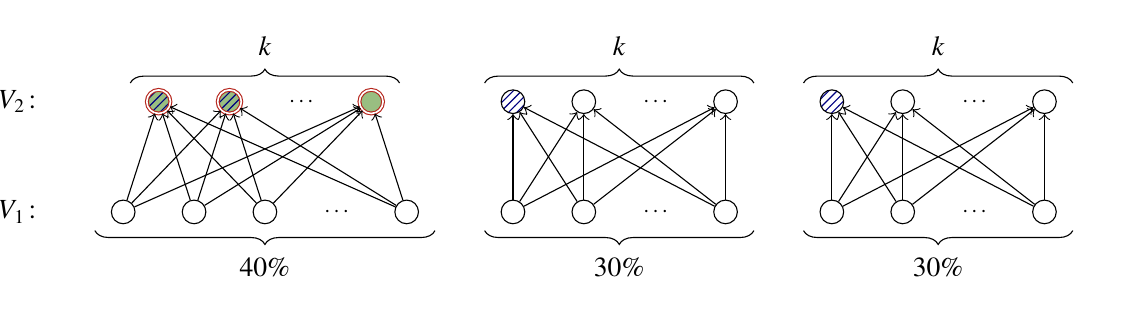
\begin{tikzpicture}[x=0.9cm,y=1.4cm] % change these values to adjust the size of a figure
	\hspace{-0.5cm}
  \tikzset{     
    e4c node/.style={circle,draw,minimum size=0.3cm,inner sep=0,font=\footnotesize}, 
    e4c edge/.style={sloped,above,font=\footnotesize}
  }
  \def\mid{5.5}
  \def\last{10}
  \node (V1) at (-0.5, 0.00) {$V_1\!:$};
  \node (V2) at (-0.5, 1.00) {$V_2\!:$};
  \node[e4c node] (1) at (1.00, 0.00) {}; 
  \node[e4c node] (2) at (2.00, 0.00) {}; 
  \node[e4c node] (3) at (3.00, 0.00) {}; 
  \node[e4c node,draw=none] (4) at (4.00, 0.00) {\ $\dots$}; 
  \node[e4c node] (5) at (5.00, 0.00) {}; 
  \node[e4c node] (6) at (1.00 + \mid, 0.00) {}; 
  \node[e4c node] (7) at (2.00 + \mid, 0.00) {}; 
  \node[e4c node,draw=none] (8) at (3.00 + \mid, 0.00) {\ $\dots$}; 
  \node[e4c node] (9) at (4.00 + \mid, 0.00) {}; 
  \node[e4c node] (10) at (1.00 + \last, 0.00) {}; 
  \node[e4c node] (11) at (2.00 + \last, 0.00) {}; 
  \node[e4c node,draw=none] (12) at (3.00 + \last, 0.00) {\ $\dots$}; 
  \node[e4c node] (13) at (4.00 + \last, 0.00) {}; 
  
  \node[e4c node,selected,selected2,selected3] (c1) at (1.50, 1.00) {}; 
  \node[e4c node,selected,selected2,selected3] (c2) at (2.50, 1.00) {}; 
  \node[e4c node,draw=none] (c123) at (3.50, 1.00) {\ $\dots$}; 
  \node[e4c node,selected,selected2] (c3) at (4.50, 1.00) {};
   

  \node[e4c node,selected3] (c4) at (1.00 + \mid, 1.00) {}; 
  \node[e4c node] (c5) at (2.00 + \mid, 1.00) {}; 
  \node[e4c node,draw=none] (c456) at (3.00 + \mid, 1.00) {\ $\dots$}; 
  \node[e4c node] (c6) at (4.00 + \mid, 1.00) {}; 
  
  \node[e4c node,selected3] (c7) at (1.00 + \last, 1.00) {}; 
  \node[e4c node] (c8) at (2.00 + \last, 1.00) {}; 
  \node[e4c node,draw=none] (c789) at (3.00 + \last, 1.00) {\ $\dots$}; 
  \node[e4c node] (c9) at (4.00 + \last, 1.00) {}; 

  \draw [decorate,decoration={brace,amplitude=5pt,mirror,raise=1.5ex}]
  	(0.6,0) -- (5.4,0) node[midway,yshift=-20]{$40\%$};
  \draw [decorate,decoration={brace,amplitude=5pt,mirror,raise=1.5ex}]
  	(0.6 + \mid,0) -- (4.4 + \mid,0) node[midway,yshift=-20]{$30\%$};
  \draw [decorate,decoration={brace,amplitude=5pt,mirror,raise=1.5ex}]
  	(0.6 + \last,0) -- (4.4 + \last,0) node[midway,yshift=-20]{$30\%$};

  \draw [decorate,decoration={brace,amplitude=5pt,raise=1.5ex}]
  	(1.1,1) -- (4.9,1) node[midway,yshift=20]{$k$};
  \draw [decorate,decoration={brace,amplitude=5pt,raise=1.5ex}]
  	(0.6 + \mid,1) -- (4.4 + \mid,1) node[midway,yshift=20]{$k$};
  \draw [decorate,decoration={brace,amplitude=5pt,raise=1.5ex}]
  	(0.6 + \last,1) -- (4.4 + \last,1) node[midway,yshift=20]{$k$};

  \path[e4c path]
  (1) edge[e4c edge]  (c1)
  (2) edge[e4c edge]  (c1)
  (3) edge[e4c edge]  (c1)
  (5) edge[e4c edge]  (c1)
  (1) edge[e4c edge]  (c2)
  (2) edge[e4c edge]  (c2)
  (3) edge[e4c edge]  (c2)
  (5) edge[e4c edge]  (c2)
  (1) edge[e4c edge]  (c3)
  (2) edge[e4c edge]  (c3)
  (3) edge[e4c edge]  (c3)
  (5) edge[e4c edge]  (c3)
  
  (6) edge[e4c edge]  (c4)
  (7) edge[e4c edge]  (c4)
  (9) edge[e4c edge]  (c4)
  (6) edge[e4c edge]  (c5)
  (7) edge[e4c edge]  (c5)
  (9) edge[e4c edge]  (c5)
  (6) edge[e4c edge]  (c6)
  (7) edge[e4c edge]  (c6)
  (9) edge[e4c edge]  (c6)
  (10) edge[e4c edge]  (c7)
  (11) edge[e4c edge]  (c7)
  (13) edge[e4c edge]  (c7)
  (10) edge[e4c edge]  (c8)
  (11) edge[e4c edge]  (c8)
  (13) edge[e4c edge]  (c8)
  (10) edge[e4c edge]  (c9)
  (11) edge[e4c edge]  (c9)
  (13) edge[e4c edge]  (c9)
  ;
\end{tikzpicture}
	\caption{
		Selecting $k$ nodes from a bipartite graph. 
		\toprank (\textcolor{BrickRed}{red} double lines) and \absorbrank (\textcolor{OliveGreen}{green} shading) select $k$ nodes from the first group of $V_2$. \mesrank (\textcolor{NavyBlue}{blue} pattern) selects $0.4k$ of nodes from the first group and $0.3k$ from each other group of $V_2$.}
	\label{fig:voting}
\end{figure}


\subsection{Bipartite Graphs}\label{sec:bipartite}
We begin with directed bipartite graphs that are particularly able to highlight the differences between measures based on PageRank and Katz centrality, as well as the characteristic behavior of proportional election rules combined with network centrality measures.
We assume that more than $k$ nodes have incoming edges; otherwise, the examined problem becomes trivial. 
Since there are only walks of length $0$ and $1$, the Katz centrality and PageRank of each node $v$ can be easily determined. Specifically, if $v$ belongs to $V_1$, its centrality is minimal, i.e., $\prm^{\alpha}_G(v) = \katz^{\alpha}_G(v) = 1.$  
Conversely, if $v$ belongs to $V_2$, then:  
\[ \prm^{\alpha}_G(v) = 1 + \sum_{(u, v) \in E} \frac{\alpha}{\deg^+(u)}, \quad \katz^{\alpha}_G(v) = 1 + \alpha \cdot \deg^-_G(v). \]  
In words, nodes in $V_2$ get $\alpha$ per incoming edge under Katz centrality, and $\alpha$ divided by the number of outgoing edges of each supporting voter under PageRank.  
As a result, \topkatz simplifies to Approval Voting in this election instance, and \toprank simplifies to Satisfaction Approval Voting.
 We highlight that since "candidate" nodes in $V_2$ have no outgoing edges, \absorbkatz and \absorbrank yield the same results as \topkatz and \toprank, respectively. 

The approach based on the Method of Equal Shares works differently. The utility that node $u$ gets from selecting node $v$ is $\mu^{\alpha}_G(u, v) = \alpha / \deg^+(u)$ for PageRank and $\mu^{\alpha}_G(u, v) = \alpha$ for Katz centrality. Consequently, \meskatz corresponds to the result of running MES when all non-zero utilities are equal to $\alpha$, while \mesrank splits $\alpha$ among all approved by $u$ candidates. 
For a visualization, consider the bipartite graph depicted in \Cref{fig:voting}. 
Methods that select nodes based on the highest PageRank or Katz centrality will choose all $k$ nodes from the first group of $V_2$, ignoring the votes of the remaining $60\%$ of voters. On the other hand, \mesrank and \meskatz will select $0.4k$ nodes from the first group and $0.3k$ nodes from each other group of $V_2$ (up to rounding). This follows from the EJR property~\citep{Peters:Skowron:2020} saying that any large enough group approving the same set of candidates should get a proportional representation.
We discuss similar axioms for our setting in \cref{sec:axioms}.

\subsection{Functional Graphs} 
\label{sec:functional} 
We now consider graphs in which every node has out-degree of at most one.  
PageRank and Katz centralities are identical on such graphs, hence, for ease of exposition, our analysis will center on rules based on PageRank.
For simplicity, we assume that the decay factor approaches 1 for all considered rules: $\alpha \rightarrow 1$.  
In this case, if a node does not lie on any cycle, the PageRank of a node is nearly equal to its number of predecessors.  
More precisely, if $|Pred(u)| > |Pred(v)|$, then $PR^{\alpha \rightarrow 1}_G(u) > PR^{\alpha \rightarrow 1}_G(v)$.

We begin with an analysis of paths.
Consider a path of length $n$, and say that $n$ is divisible by $k$.  
$\mesrank$ views this instance as an election in which every node receives a utility of approximately $1$ from each predecessor.  
Hence it selects the last $k$ nodes of the path, as they have the maximum number of predecessors, clearly dominating the other nodes.
The same holds for \toprank.
However, $\absorbrank$ behaves differently. 
The sink of the path will be again selected, but then, 
if the second-to-last node is selected, the sink will have no incoming edges in the graph $G - E^+(S)$, and its PageRank will be minimized.  
Therefore, the rule avoids such a selection.  
Instead, it aims to select nodes in such a way that they have equal support in the graph without their outgoing edges: it selects nodes $\nicefrac{n}{k}, 2 \cdot \nicefrac{n}{k}, \dots, n$.  
For an illustration we refer to \Cref{fig:paths}.


\begin{figure}[t]
	\centering
	
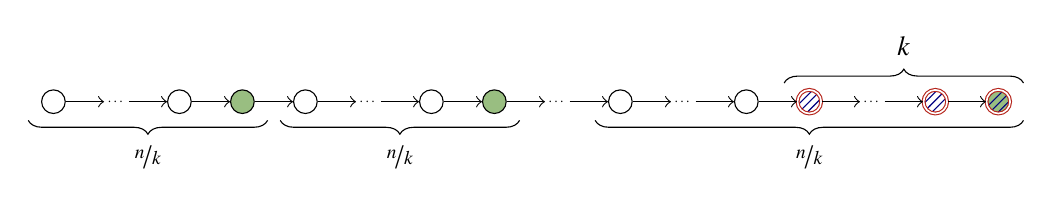
\begin{tikzpicture}[scale=1]
  \def\y{0}
  \def\x{0.8}
  \node[e4c node] (1) at (1.00*\x, \y) {}; 
  \node[e4c node,draw=none] (2) at (2.00*\x, \y) {$\dots$}; 
  \node[e4c node] (3) at (3.00*\x, \y) {}; 
  \node[e4c node,selected2] (4) at (4.00*\x, \y) {}; 
  
  \node[e4c node] (5) at (5.00*\x, \y) {}; 
  \node[e4c node,draw=none] (6) at (6.00*\x, \y) {$\dots$}; 
  \node[e4c node] (7) at (7.00*\x, \y) {}; 
  \node[e4c node,selected2] (8) at (8.00*\x, \y) {}; 

  \node[e4c node,draw=none] (9) at (9.00*\x, \y) {$\dots$}; 
  
  \node[e4c node] (10) at (10.00*\x, \y) {}; 
  \node[e4c node,draw=none] (11) at (11.00*\x, \y) {$\dots$}; 
  \node[e4c node] (12) at (12.00*\x, \y) {}; 
  \node[e4c node,selected,selected3] (13) at (13.00*\x, \y) {}; 
  \node[e4c node,draw=none] (14) at (14.00*\x, \y) {$\dots$}; 
  \node[e4c node,selected,selected3] (15) at (15.00*\x, \y) {}; 
  \node[e4c node,selected,selected2,selected3] (16) at (16.00*\x, \y) {}; 

  \draw [decorate,decoration={brace,amplitude=5pt,mirror,raise=1.5ex}]
  	(0.6*\x,\y) -- (4.4*\x,\y) node[midway,yshift=-20]{$\nicefrac{n}{k}$};
  \draw [decorate,decoration={brace,amplitude=5pt,mirror,raise=1.5ex}]
  	(4.6*\x,\y) -- (8.4*\x,\y) node[midway,yshift=-20]{$\nicefrac{n}{k}$};
  \draw [decorate,decoration={brace,amplitude=5pt,mirror,raise=1.5ex}]
  	(9.6*\x,\y) -- (16.4*\x,\y) node[midway,yshift=-20]{$\nicefrac{n}{k}$};
  	
  \draw [decorate,decoration={brace,amplitude=5pt,raise=1.5ex}]
  	(12.6*\x,\y) -- (16.4*\x,\y) node[midway,yshift=20]{$k$};
 	

  \path[e4c path]
  (1) edge[e4c edge]  (2)
  (2) edge[e4c edge]  (3)
  (3) edge[e4c edge]  (4)
  (4) edge[e4c edge]  (5)
  (5) edge[e4c edge]  (6)
  (6) edge[e4c edge]  (7)
  (7) edge[e4c edge]  (8)
  (8) edge[e4c edge]  (9)
  (9) edge[e4c edge]  (10)
  (10) edge[e4c edge]  (11)
  (11) edge[e4c edge]  (12)
  (12) edge[e4c edge]  (13)
  (13) edge[e4c edge]  (14)
  (14) edge[e4c edge]  (15)
  (15) edge[e4c edge]  (16)
  ;
  
\end{tikzpicture}	
	\caption{Selecting $k$ nodes from the $n$-path ($n$ divisible by $k$).
	\textsc{Top}-\textsc{Rank} (\textcolor{BrickRed}{red} double lines) and \mesrank (\textcolor{NavyBlue}{blue} pattern) choose the last $k$ nodes.
	\absorbrank (\textcolor{OliveGreen}{green} shading) selects nodes evenly splitting the path.}
	\label{fig:paths}
\end{figure}


Consider now an arbitrary (connected) functional graph.
Observe that such a graph consists of at most one cycle and in-trees attached to nodes from the cycle.
Nodes from the cycle clearly have the maximal PageRank and have non-zero (close to $1$) utility for all the nodes.
Thus, if the cycle contains at least $k$ nodes, then both \toprank and \mesrank would select only nodes from the cycle.
If not, both methods select all nodes from the cycle and then some nodes from the attached in-trees.
This is, however, where both methods begin to differ, and we refer to \Cref{fig:functional} for a specific example. \toprank will select nodes with the highest number of predecessors. All such nodes may come from the same in-tree.
However, from each in-tree \mesrank will select a number of nodes proportional to its size.
Let us switch our attention to \absorbrank. 
If the graph contains a cycle, then \absorbrank would select one node from the cycle, say $v$.
The graph $G - E^+(v)$ is a tree.
Hence, roughly speaking, \absorbrank splits this tree into parts of equal size, and from each part selects its root.

The analysis of functional graphs
shows an important difference in how \absorbrank and \mesrank interpret proportionality.




\begin{figure}
	\centering
%	\begin{tikzpicture}[every node/.style={draw, circle, minimum size=4mm}]
%		% Nodes with correct pattern fills
%		\node[pattern=vertical lines] (R) at (0,2) {};
%		\node[pattern=horizontal lines] (Re) at (0,2) {};
%		\node[pattern=vertical lines] (A) at (-1,1) {};
%		\node[pattern=horizontal lines] (B) at (1,1) {};
%		
%		% Create leaf nodes
%		\node (A1) at (-1.5,0) {};
%		\node (A2) at (-0.5,0) {};
%		
%		\node (B1) at (0.5,0) {};
%		\node (B2) at (1.5,0) {};
%		
%		% Edges
%		\draw[->] (A) -- (R);
%		\draw[->] (B) -- (R);
%		\draw[->] (A1) -- (A);
%		\draw[->] (A2) -- (A);
%		\draw[->] (B1) -- (B);
%		\draw[->] (B2) -- (B1);
%	\end{tikzpicture}
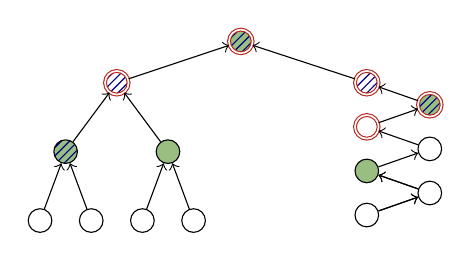
\begin{tikzpicture}[x=5cm, y=3.5cm] % change these values to adjust the size of a figure
  \node[e4c node,selected,selected2,selected3] (1) at (0.51, 1.50) {}; 
  \node[e4c node,selected,selected3] (2) at (0.195, 1.35) {}; 
  \node[e4c node,selected2,selected3] (3) at (0.065, 1.10) {}; 
  \node[e4c node,selected2] (4) at (0.325, 1.10) {}; 
  \node[e4c node] (5) at (0.00, 0.85) {}; 
  \node[e4c node] (6) at (0.13, 0.85) {}; 
  \node[e4c node] (7) at (0.26, 0.85) {}; 
  \node[e4c node] (8) at (0.39, 0.85) {}; 
  \node[e4c node,selected,selected3] (9) at (0.83, 1.35) {}; 
  \node[e4c node,selected,selected2,selected3] (10) at (0.99, 1.27) {}; 
  \node[e4c node,selected] (11) at (0.83, 1.19) {}; 
  \node[e4c node] (12) at (0.99, 1.11) {}; 
  \node[e4c node,selected2] (13) at (0.83, 1.03) {}; 
  \node[e4c node] (14) at (0.99, 0.95) {}; 
  \node[e4c node] (15) at (0.83, 0.87) {}; 

  \path[e4c path]
  (15) edge[e4c edge]  (14)
  (14) edge[e4c edge]  (13)
  (2) edge[e4c edge]  (1)
  (3) edge[e4c edge]  (2)
  (4) edge[e4c edge]  (2)
  (5) edge[e4c edge]  (3)
  (6) edge[e4c edge]  (3)
  (7) edge[e4c edge]  (4)
  (8) edge[e4c edge]  (4)
  (9) edge[e4c edge]  (1)
  (10) edge[e4c edge]  (9)
  (11) edge[e4c edge]  (10)
  (12) edge[e4c edge]  (11)
  (13) edge[e4c edge]  (12)
  (14) edge[e4c edge]  (13)
  (15) edge[e4c edge]  (14)
  ;
\end{tikzpicture}
	\caption{Selecting $k=5$ nodes from a (directed in-)tree with two unbalanced branches of equal size. \toprank (\textcolor{BrickRed}{red} double lines) selects mostly from the right-hand side. \mesrank (\textcolor{NavyBlue}{blue} pattern) selects two nodes from each side. \absorbrank (\textcolor{OliveGreen}{green} shading) splits the tree in subtrees of size $3$.}
	\label{fig:functional}
\end{figure}

\section{Axioms of Proportionality}
\label{sec:axioms}

We now introduce axioms to formalize the intuition that a sufficiently large and cohesive group of nodes deserves a proportional number of representatives. Our results (depicted in 
\Cref{table:axioms}) shed further light on the differences among the examined rules. Specifically, our axioms are inspired by the literature on multiwinner election rules. 
Following the approach from works in this area (e.g., \citep{aziz2017justified}), the idea is that each node should have a significant influence over $\nicefrac{k}{n}$ of the committee.
Consequently, a cohesive group $S$ is entitled to $\lfloor k \cdot \nicefrac{|S|}{n} \rfloor$ representatives. 
The key question, then, is: in the context of our study, which groups of nodes can be considered cohesive, and which nodes qualify as proper representatives of these groups?


We view a group of nodes as cohesive if all nodes mutually approve each other, either directly or indirectly. 
In graph terms, this means the group induces a strongly connected subgraph. 
We do so because in such groups, the importance is, to some extent, evenly distributed among its members.
%
The most cohesive groups of nodes possible
are the ones that form a component that is a clique.
Our first axiom states that each such a component
is entitled to a representation
proportional to its size.

\medskip
\noindent\textbf{Clique-Entitlement:}  
For every graph $G = (V, E)$,  
if there exists a strongly connected component $S \subseteq V$  
such that $G[S]$ is a clique,  
then $|S \cap \mathcal{R}(G, k)| \ge \lfloor k \cdot \nicefrac{|S|}{n} \rfloor$.  
 \medskip
 
\toprank and \topkatz do not satisfy this axiom,
as they may overlook nodes from a clique component 
that should receive a representation
when a larger and more diverse component exists.
In contrast,
we will later show that \absorbrank, \mesrank, and \meskatz satisfy this axiom. 

\begin{table}[t]
	\centering
	\begin{tabular}{ccc|l}
		\toprule
		Clique- & Component- & Subgraph- & Entitlement \\
		\midrule
		\no & \no & \no & \topkatz /\toprank \\
		\no & \no & \no & \absorbkatz\\
		\yes & \no & \no & \absorbrank\\
		\yes & \yes & \yes & \meskatz /\mesrank\\
				\bottomrule
	\end{tabular}
	\caption{Summary of the axiomatic properties.}
	\label{table:axioms}
\end{table}

\begin{proposition} 
	\label{prop:axioms_topk}
	\toprank and \topkatz do not satisfy Clique-Entitlement.
\end{proposition}

Next, we generalize Clique-Entitlement and require only that the component is strongly connected.
It turns out that \absorbrank doesn't satisfy this stronger axiom, in contrast to \mesrank and \meskatz.

\medskip
\noindent\textbf{Component-Entitlement:}  
For every graph $G = (V, E)$,  
if there exists a strongly connected component $S \subseteq V$,  
then $|S \cap \mathcal{R}(G, k)| \ge \lfloor k \cdot \nicefrac{|S|}{n} \rfloor$.  
\medskip

Recall that \absorbrank attempts to divide the graph $G$ into equal parts to maximize the minimal PageRank in $G-E(S\!)$ among nodes in $S\!$. 
Given this, \absorbrank violates Component-Entitlement because, depending on the structure, some components may be easier or harder to divide into several equal parts. 
As a result, it might be more beneficial to select an additional node from one component rather than another.
Interestingly, \absorbkatz not only fails this axiom but also Clique-Entitlement, which highlights a crucial difference between the two absorbing methods.
\begin{theorem} 
\label{prop:axioms_absorb}
\absorbrank satisfies Clique-Entitlement, but does not satisfy Component-Entitlement. 
\absorbkatz does not satisfy Clique-Entitlement.
\end{theorem}

On the other hand, \mesrank and \meskatz also satisfy a stronger property.
Consider an arbitrary strongly connected subgraph within a larger component of a graph.
Since this subgraph is not entirely separate from other nodes, its delegated votes may flow outside the group. However, these votes will always flow to their successors.
In the previous axioms, we assumed that a group deserving representation would be represented by its own members. 
In contrast, we now allow for representation through successors.


\medskip
\noindent\textbf{Subgraph-Entitlement:}
For every graph $G=(V,E)$,
if there exists a subset of nodes $S \subseteq V$ 
such that $G[S]$ is strongly connected, then
$|(S \cup \Succ(S)) \cap \mathcal{R}(G,k)| \ge \lfloor k \cdot \nicefrac{|S|}{n} \rfloor$.
\medskip

It is straightforward to observe that Subgraph-Entitlement implies Component-Entitlement, and, in turn, Clique-Entitlement. 
Consequently, Subgraph-Entitlement is violated by \toprank, \absorbrank, and their variants.  
Our positive result for \mesrank and \meskatz is even more general, as it applies to all selection rules based on the Method of Equal Shares and any centrality measure that satisfies a basic consistency condition: the utility of a node $u$ from a node $v$ is non-zero if and only if 
$u$ transfers a fraction of its vote to $v$, at least indirectly.

\begin{samepage}
\begin{theorem}
\label{prop:axioms_mes}
Assume that a utility function $\mu_G$ satisfies $\mu_G(u, v) > 0$ if and only if there is a path from $u$ to $v$.  
Applying the Method of Equal Shares for such a utility function results in a rule satisfying Subgraph-Entitlement.
In particular, \mesrank and \meskatz satisfy this property.
\end{theorem}
\end{samepage}


\section{Experiments}
\label{sec:experiments}


In this section, we compare \toprank, \seqabsorbrank, and \mesrank, along with their Katz counterparts, empircally,
on both real-life and synthetic data. 
Additionally, we include \bosrank and \boskatz, defined similarly to \mesrank and \meskatz but using the fine-tuned variant of MES called the Method of Equal Shares with Bounded Overspending (BOS)~\citep{papasotiropoulos2024method}. This is argued to better handle data with high variance in candidate utilities, a common characteristic of our model.
We set $\alpha=0.85$ for PageRank-based rules, as used by \cite{brin1998anatomy}, and $\alpha=0.85/\lambda$ for 
Katz-based ones.
First, we analyze two network datasets often used as benchmarks for community detection algorithms~\citep{jin2021survey}.

\subsection{College Football Network}\label{sec:college-football-network}
The first dataset \citep{GirNew-2002-CommunityDetection} is a graph of 115 nodes representing U.S. college football teams.
Each undirected edge denotes a game played in Division IA during the 2000 Fall season (see \cref{fig:football:graph}).
We interpet each such undirected edge as a pair of directed edges in both directions.
The teams are split into 11 conferences and a group of independents.
Around 64\% of games occur within the conferences
and the rest are played across them.

\begin{figure}[t]
	\centering
 \scalebox{1}{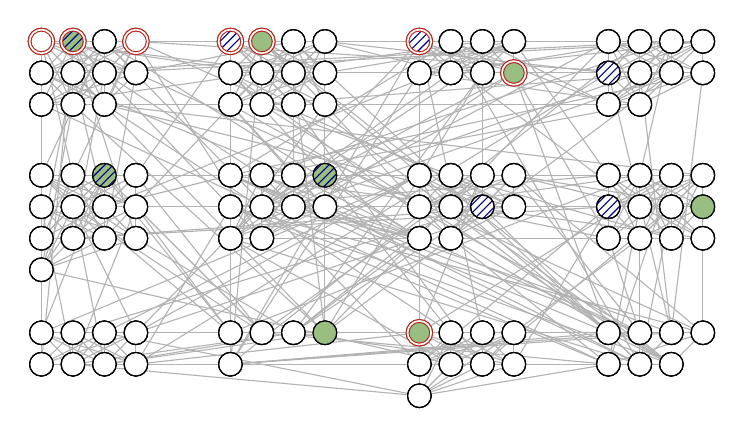
\begin{tikzpicture}
  \def\x{0.4}
  \def\y{0.4}
  \def\xx{2.4}
  \def\yyzero{0}
  \def\yyone{1.7}
  \def\yytwo{3.7}
  \node[e4c node,selected,selected2] (BrighamYoung) at (0*\x + 2*\xx, -0*\y - \yyzero) {};
  \node[e4c node,selected,selected3] (FloridaState) at (0*\x + 2*\xx, -0*\y - \yytwo) {};
  \node[e4c node,selected] (Iowa) at (0*\x + 0*\xx, -0*\y - \yyzero) {};
  \node[e4c node,selected,selected2] (KansasState) at (0*\x + 1*\xx, -0*\y - \yyzero) {};
  \node[e4c node] (NewMexico) at (1*\x + 2*\xx, -0*\y - \yyzero) {};
  \node[e4c node,selected,selected3] (TexasTech) at (1*\x + 1*\xx, -0*\y - \yyzero) {};
  \node[e4c node,selected,selected2,selected3] (PennState) at (1*\x + 0*\xx, -0*\y - \yyzero) {};
  \node[e4c node] (SouthernCalifornia) at (0*\x + 3*\xx, -0*\y - \yyzero) {};
  \node[e4c node] (ArizonaState) at (1*\x + 3*\xx, -0*\y - \yyzero) {};
  \node[e4c node] (SanDiegoState) at (2*\x + 2*\xx, -0*\y - \yyzero) {};
  \node[e4c node] (Baylor) at (2*\x + 1*\xx, -0*\y - \yyzero) {};
  \node[e4c node] (NorthTexas) at (0*\x + 3*\xx, -0*\y - \yytwo) {};
  \node[e4c node] (NorthernIllinois) at (0*\x + 0*\xx, -0*\y - \yyone) {};
  \node[e4c node] (Northwestern) at (2*\x + 0*\xx, -0*\y - \yyzero) {};
  \node[e4c node] (WesternMichigan) at (1*\x + 0*\xx, -0*\y - \yyone) {};
  \node[e4c node,selected] (Wisconsin) at (3*\x + 0*\xx, -0*\y - \yyzero) {};
  \node[e4c node] (Wyoming) at (3*\x + 2*\xx, -0*\y - \yyzero) {};
  \node[e4c node] (Auburn) at (0*\x + 3*\xx, -0*\y - \yyone) {};
  \node[e4c node,selected2,selected3] (Akron) at (2*\x + 0*\xx, -0*\y - \yyone) {};
  \node[e4c node] (VirginiaTech) at (0*\x + 0*\xx, -0*\y - \yytwo) {};
  \node[e4c node] (Alabama) at (1*\x + 3*\xx, -0*\y - \yyone) {};
  \node[e4c node] (UCLA) at (2*\x + 3*\xx, -0*\y - \yyzero) {};
  \node[e4c node] (Arizona) at (3*\x + 3*\xx, -0*\y - \yyzero) {};
  \node[e4c node] (Utah) at (0*\x + 2*\xx, -1*\y - \yyzero) {};
  \node[e4c node] (ArkansasState) at (1*\x + 3*\xx, -0*\y - \yytwo) {};
  \node[e4c node] (NorthCarolinaState) at (1*\x + 2*\xx, -0*\y - \yytwo) {};
  \node[e4c node] (BallState) at (3*\x + 0*\xx, -0*\y - \yyone) {};
  \node[e4c node] (Florida) at (2*\x + 3*\xx, -0*\y - \yyone) {};
  \node[e4c node] (BoiseState) at (0*\x + 1*\xx, -0*\y - \yyone) {};
  \node[e4c node] (BostonCollege) at (1*\x + 0*\xx, -0*\y - \yytwo) {};
  \node[e4c node] (WestVirginia) at (2*\x + 0*\xx, -0*\y - \yytwo) {};
  \node[e4c node] (BowlingGreenState) at (0*\x + 0*\xx, -1*\y - \yyone) {};
  \node[e4c node] (Michigan) at (0*\x + 0*\xx, -1*\y - \yyzero) {};
  \node[e4c node] (Virginia) at (2*\x + 2*\xx, -0*\y - \yytwo) {};
  \node[e4c node] (Buffalo) at (1*\x + 0*\xx, -1*\y - \yyone) {};
  \node[e4c node] (Syracuse) at (3*\x + 0*\xx, -0*\y - \yytwo) {};
  \node[e4c node] (CentralFlorida) at (0*\x + 1*\xx, -0*\y - \yytwo) {};
  \node[e4c node] (GeorgiaTech) at (3*\x + 2*\xx, -0*\y - \yytwo) {};
  \node[e4c node] (CentralMichigan) at (2*\x + 0*\xx, -1*\y - \yyone) {};
  \node[e4c node] (Purdue) at (1*\x + 0*\xx, -1*\y - \yyzero) {};
  \node[e4c node] (Colorado) at (3*\x + 1*\xx, -0*\y - \yyzero) {};
  \node[e4c node] (ColoradoState) at (1*\x + 2*\xx, -1*\y - \yyzero) {};
  \node[e4c node] (Connecticut) at (1*\x + 1*\xx, -0*\y - \yytwo) {};
  \node[e4c node] (EasternMichigan) at (3*\x + 0*\xx, -1*\y - \yyone) {};
  \node[e4c node] (EastCarolina) at (0*\x + 2*\xx, -0*\y - \yyone) {};
  \node[e4c node] (Duke) at (0*\x + 2*\xx, -1*\y - \yytwo) {};
  \node[e4c node] (FresnoState) at (1*\x + 1*\xx, -0*\y - \yyone) {};
  \node[e4c node] (OhioState) at (2*\x + 0*\xx, -1*\y - \yyzero) {};
  \node[e4c node] (Houston) at (1*\x + 2*\xx, -0*\y - \yyone) {};
  \node[e4c node] (Rice) at (2*\x + 1*\xx, -0*\y - \yyone) {};
  \node[e4c node] (Idaho) at (2*\x + 3*\xx, -0*\y - \yytwo) {};
  \node[e4c node,selected2] (Washington) at (0*\x + 3*\xx, -1*\y - \yyzero) {};
  \node[e4c node] (Kansas) at (0*\x + 1*\xx, -1*\y - \yyzero) {};
  \node[e4c node,selected2,selected3] (SouthernMethodist) at (3*\x + 1*\xx, -0*\y - \yyone) {};
  \node[e4c node] (Kent) at (0*\x + 0*\xx, -2*\y - \yyone) {};
  \node[e4c node] (Pittsburgh) at (0*\x + 0*\xx, -1*\y - \yytwo) {};
  \node[e4c node] (Kentucky) at (3*\x + 3*\xx, -0*\y - \yyone) {};
  \node[e4c node] (Louisville) at (2*\x + 2*\xx, -0*\y - \yyone) {};
  \node[e4c node] (LouisianaTech) at (0*\x + 1*\xx, -1*\y - \yyone) {};
  \node[e4c node] (LouisianaMonroe) at (3*\x + 3*\xx, -0*\y - \yytwo) {};
  \node[e4c node] (Minnesota) at (3*\x + 0*\xx, -1*\y - \yyzero) {};
  \node[e4c node] (MiamiOhio) at (1*\x + 0*\xx, -2*\y - \yyone) {};
  \node[e4c node,selected2] (Vanderbilt) at (0*\x + 3*\xx, -1*\y - \yyone) {};
  \node[e4c node] (MiddleTennesseeState) at (0*\x + 3*\xx, -1*\y - \yytwo) {};
  \node[e4c node] (Illinois) at (0*\x + 0*\xx, -2*\y - \yyzero) {};
  \node[e4c node] (MississippiState) at (1*\x + 3*\xx, -1*\y - \yyone) {};
  \node[e4c node] (Memphis) at (3*\x + 2*\xx, -0*\y - \yyone) {};
  \node[e4c node] (Nevada) at (1*\x + 1*\xx, -1*\y - \yyone) {};
  \node[e4c node] (Oregon) at (1*\x + 3*\xx, -1*\y - \yyzero) {};
  \node[e4c node] (NewMexicoState) at (1*\x + 3*\xx, -1*\y - \yytwo) {};
  \node[e4c node] (SouthCarolina) at (2*\x + 3*\xx, -1*\y - \yyone) {};
  \node[e4c node] (Ohio) at (2*\x + 0*\xx, -2*\y - \yyone) {};
  \node[e4c node] (IowaState) at (1*\x + 1*\xx, -1*\y - \yyzero) {};
  \node[e4c node] (SanJoseState) at (2*\x + 1*\xx, -1*\y - \yyone) {};
  \node[e4c node] (Nebraska) at (2*\x + 1*\xx, -1*\y - \yyzero) {};
  \node[e4c node] (SouthernMississippi) at (0*\x + 2*\xx, -1*\y - \yyone) {};
  \node[e4c node,selected3] (Tennessee) at (3*\x + 3*\xx, -1*\y - \yyone) {};
  \node[e4c node] (Stanford) at (2*\x + 3*\xx, -1*\y - \yyzero) {};
  \node[e4c node] (WashingtonState) at (3*\x + 3*\xx, -1*\y - \yyzero) {};
  \node[e4c node] (Temple) at (1*\x + 0*\xx, -1*\y - \yytwo) {};
  \node[e4c node] (Navy) at (2*\x + 1*\xx, -0*\y - \yytwo) {};
  \node[e4c node] (TexasA&M) at (3*\x + 1*\xx, -1*\y - \yyzero) {};
  \node[e4c node,selected3] (NotreDame) at (3*\x + 1*\xx, -0*\y - \yytwo) {};
  \node[e4c node] (TexasElPaso) at (3*\x + 1*\xx, -1*\y - \yyone) {};
  \node[e4c node] (Oklahoma) at (0*\x + 1*\xx, -2*\y - \yyzero) {};
  \node[e4c node] (Toledo) at (3*\x + 0*\xx, -2*\y - \yyone) {};
  \node[e4c node] (Tulane) at (1*\x + 2*\xx, -1*\y - \yyone) {};
  \node[e4c node] (Mississippi) at (0*\x + 3*\xx, -2*\y - \yyone) {};
  \node[e4c node] (Tulsa) at (0*\x + 1*\xx, -2*\y - \yyone) {};
  \node[e4c node] (NorthCarolina) at (1*\x + 2*\xx, -1*\y - \yytwo) {};
  \node[e4c node] (UtahState) at (0*\x + 1*\xx, -1*\y - \yytwo) {};
  \node[e4c node,selected2] (Army) at (2*\x + 2*\xx, -1*\y - \yyone) {};
  \node[e4c node] (Cincinnati) at (3*\x + 2*\xx, -1*\y - \yyone) {};
  \node[e4c node] (AirForce) at (2*\x + 2*\xx, -1*\y - \yyzero) {};
  \node[e4c node] (Rutgers) at (2*\x + 0*\xx, -1*\y - \yytwo) {};
  \node[e4c node] (Georgia) at (1*\x + 3*\xx, -2*\y - \yyone) {};
  \node[e4c node] (LouisianaState) at (2*\x + 3*\xx, -2*\y - \yyone) {};
  \node[e4c node] (LouisianaLafayette) at (2*\x + 3*\xx, -1*\y - \yytwo) {};
  \node[e4c node] (Texas) at (1*\x + 1*\xx, -2*\y - \yyzero) {};
  \node[e4c node] (Marshall) at (0*\x + 0*\xx, -3*\y - \yyone) {};
  \node[e4c node] (MichiganState) at (1*\x + 0*\xx, -2*\y - \yyzero) {};
  \node[e4c node] (MiamiFlorida) at (3*\x + 0*\xx, -1*\y - \yytwo) {};
  \node[e4c node] (Missouri) at (2*\x + 1*\xx, -2*\y - \yyzero) {};
  \node[e4c node] (Clemson) at (2*\x + 2*\xx, -1*\y - \yytwo) {};
  \node[e4c node,selected,selected3] (NevadaLasVegas) at (3*\x + 2*\xx, -1*\y - \yyzero) {};
  \node[e4c node] (WakeForest) at (3*\x + 2*\xx, -1*\y - \yytwo) {};
  \node[e4c node] (Indiana) at (2*\x + 0*\xx, -2*\y - \yyzero) {};
  \node[e4c node] (OklahomaState) at (3*\x + 1*\xx, -2*\y - \yyzero) {};
  \node[e4c node] (OregonState) at (0*\x + 3*\xx, -2*\y - \yyzero) {};
  \node[e4c node] (Maryland) at (0*\x + 2*\xx, -2*\y - \yytwo) {};
  \node[e4c node] (TexasChristian) at (0*\x + 2*\xx, -2*\y - \yyone) {};
  \node[e4c node] (California) at (1*\x + 3*\xx, -2*\y - \yyzero) {};
  \node[e4c node] (AlabamaBirmingham) at (1*\x + 2*\xx, -2*\y - \yyone) {};
  \node[e4c node] (Arkansas) at (3*\x + 3*\xx, -2*\y - \yyone) {};
  \node[e4c node] (Hawaii) at (1*\x + 1*\xx, -2*\y - \yyone) {};

  \path[draw=black!30,thin]
  (BrighamYoung) edge (FloridaState)
  (BrighamYoung) edge (NewMexico)
  (BrighamYoung) edge (SanDiegoState)
  (BrighamYoung) edge (Wyoming)
  (BrighamYoung) edge (Utah)
  (BrighamYoung) edge (Virginia)
  (BrighamYoung) edge (Syracuse)
  (BrighamYoung) edge (ColoradoState)
  (BrighamYoung) edge (MississippiState)
  (BrighamYoung) edge (UtahState)
  (BrighamYoung) edge (AirForce)
  (BrighamYoung) edge (NevadaLasVegas)
  (FloridaState) edge (NorthCarolinaState)
  (FloridaState) edge (Florida)
  (FloridaState) edge (Virginia)
  (FloridaState) edge (GeorgiaTech)
  (FloridaState) edge (Duke)
  (FloridaState) edge (Louisville)
  (FloridaState) edge (NorthCarolina)
  (FloridaState) edge (MiamiFlorida)
  (FloridaState) edge (Clemson)
  (FloridaState) edge (WakeForest)
  (FloridaState) edge (Maryland)
  (Iowa) edge (KansasState)
  (Iowa) edge (PennState)
  (Iowa) edge (Northwestern)
  (Iowa) edge (WesternMichigan)
  (Iowa) edge (Wisconsin)
  (Iowa) edge (OhioState)
  (Iowa) edge (Minnesota)
  (Iowa) edge (Illinois)
  (Iowa) edge (IowaState)
  (Iowa) edge (Nebraska)
  (Iowa) edge (MichiganState)
  (Iowa) edge (Indiana)
  (KansasState) edge (TexasTech)
  (KansasState) edge (NorthTexas)
  (KansasState) edge (BallState)
  (KansasState) edge (Colorado)
  (KansasState) edge (Kansas)
  (KansasState) edge (LouisianaTech)
  (KansasState) edge (IowaState)
  (KansasState) edge (Nebraska)
  (KansasState) edge (TexasA&M)
  (KansasState) edge (Oklahoma)
  (KansasState) edge (Missouri)
  (NewMexico) edge (TexasTech)
  (NewMexico) edge (SanDiegoState)
  (NewMexico) edge (Wyoming)
  (NewMexico) edge (Utah)
  (NewMexico) edge (BoiseState)
  (NewMexico) edge (ColoradoState)
  (NewMexico) edge (NewMexicoState)
  (NewMexico) edge (AirForce)
  (NewMexico) edge (NevadaLasVegas)
  (NewMexico) edge (OregonState)
  (TexasTech) edge (Baylor)
  (TexasTech) edge (NorthTexas)
  (TexasTech) edge (Kansas)
  (TexasTech) edge (Nebraska)
  (TexasTech) edge (TexasA&M)
  (TexasTech) edge (Oklahoma)
  (TexasTech) edge (UtahState)
  (TexasTech) edge (LouisianaLafayette)
  (TexasTech) edge (Texas)
  (TexasTech) edge (OklahomaState)
  (PennState) edge (SouthernCalifornia)
  (PennState) edge (Michigan)
  (PennState) edge (Purdue)
  (PennState) edge (OhioState)
  (PennState) edge (Pittsburgh)
  (PennState) edge (LouisianaTech)
  (PennState) edge (Minnesota)
  (PennState) edge (Illinois)
  (PennState) edge (Toledo)
  (PennState) edge (MichiganState)
  (PennState) edge (Indiana)
  (SouthernCalifornia) edge (ArizonaState)
  (SouthernCalifornia) edge (UCLA)
  (SouthernCalifornia) edge (Arizona)
  (SouthernCalifornia) edge (Colorado)
  (SouthernCalifornia) edge (Oregon)
  (SouthernCalifornia) edge (SanJoseState)
  (SouthernCalifornia) edge (Stanford)
  (SouthernCalifornia) edge (WashingtonState)
  (SouthernCalifornia) edge (NotreDame)
  (SouthernCalifornia) edge (OregonState)
  (SouthernCalifornia) edge (California)
  (ArizonaState) edge (SanDiegoState)
  (ArizonaState) edge (UCLA)
  (ArizonaState) edge (Arizona)
  (ArizonaState) edge (ColoradoState)
  (ArizonaState) edge (Washington)
  (ArizonaState) edge (Oregon)
  (ArizonaState) edge (Stanford)
  (ArizonaState) edge (WashingtonState)
  (ArizonaState) edge (UtahState)
  (ArizonaState) edge (California)
  (SanDiegoState) edge (Wyoming)
  (SanDiegoState) edge (Arizona)
  (SanDiegoState) edge (Utah)
  (SanDiegoState) edge (ColoradoState)
  (SanDiegoState) edge (Illinois)
  (SanDiegoState) edge (AirForce)
  (SanDiegoState) edge (NevadaLasVegas)
  (SanDiegoState) edge (OregonState)
  (Baylor) edge (NorthTexas)
  (Baylor) edge (Minnesota)
  (Baylor) edge (IowaState)
  (Baylor) edge (Nebraska)
  (Baylor) edge (TexasA&M)
  (Baylor) edge (Oklahoma)
  (Baylor) edge (Texas)
  (Baylor) edge (Missouri)
  (Baylor) edge (OklahomaState)
  (NorthTexas) edge (ArkansasState)
  (NorthTexas) edge (BoiseState)
  (NorthTexas) edge (Idaho)
  (NorthTexas) edge (NewMexicoState)
  (NorthTexas) edge (UtahState)
  (NorthTexas) edge (LouisianaLafayette)
  (NorthTexas) edge (NevadaLasVegas)
  (NorthernIllinois) edge (Northwestern)
  (NorthernIllinois) edge (WesternMichigan)
  (NorthernIllinois) edge (Auburn)
  (NorthernIllinois) edge (Akron)
  (NorthernIllinois) edge (BallState)
  (NorthernIllinois) edge (Buffalo)
  (NorthernIllinois) edge (CentralFlorida)
  (NorthernIllinois) edge (CentralMichigan)
  (NorthernIllinois) edge (EasternMichigan)
  (NorthernIllinois) edge (Toledo)
  (Northwestern) edge (Wisconsin)
  (Northwestern) edge (Michigan)
  (Northwestern) edge (Purdue)
  (Northwestern) edge (Duke)
  (Northwestern) edge (Minnesota)
  (Northwestern) edge (Illinois)
  (Northwestern) edge (MichiganState)
  (Northwestern) edge (Indiana)
  (Northwestern) edge (TexasChristian)
  (WesternMichigan) edge (Wisconsin)
  (WesternMichigan) edge (BallState)
  (WesternMichigan) edge (CentralMichigan)
  (WesternMichigan) edge (EasternMichigan)
  (WesternMichigan) edge (Kent)
  (WesternMichigan) edge (Ohio)
  (WesternMichigan) edge (Toledo)
  (WesternMichigan) edge (Marshall)
  (Wisconsin) edge (Michigan)
  (Wisconsin) edge (Purdue)
  (Wisconsin) edge (OhioState)
  (Wisconsin) edge (Minnesota)
  (Wisconsin) edge (Oregon)
  (Wisconsin) edge (Cincinnati)
  (Wisconsin) edge (MichiganState)
  (Wisconsin) edge (Indiana)
  (Wisconsin) edge (Hawaii)
  (Wyoming) edge (Auburn)
  (Wyoming) edge (Utah)
  (Wyoming) edge (CentralMichigan)
  (Wyoming) edge (ColoradoState)
  (Wyoming) edge (Nevada)
  (Wyoming) edge (TexasA&M)
  (Wyoming) edge (AirForce)
  (Wyoming) edge (NevadaLasVegas)
  (Auburn) edge (Alabama)
  (Auburn) edge (Florida)
  (Auburn) edge (LouisianaTech)
  (Auburn) edge (Vanderbilt)
  (Auburn) edge (MississippiState)
  (Auburn) edge (Mississippi)
  (Auburn) edge (Georgia)
  (Auburn) edge (LouisianaState)
  (Auburn) edge (Arkansas)
  (Akron) edge (VirginiaTech)
  (Akron) edge (BowlingGreenState)
  (Akron) edge (Buffalo)
  (Akron) edge (CentralFlorida)
  (Akron) edge (CentralMichigan)
  (Akron) edge (Connecticut)
  (Akron) edge (Kent)
  (Akron) edge (MiamiOhio)
  (Akron) edge (Ohio)
  (Akron) edge (Marshall)
  (VirginiaTech) edge (BostonCollege)
  (VirginiaTech) edge (WestVirginia)
  (VirginiaTech) edge (Virginia)
  (VirginiaTech) edge (Syracuse)
  (VirginiaTech) edge (CentralFlorida)
  (VirginiaTech) edge (EastCarolina)
  (VirginiaTech) edge (Pittsburgh)
  (VirginiaTech) edge (Temple)
  (VirginiaTech) edge (Rutgers)
  (VirginiaTech) edge (MiamiFlorida)
  (Alabama) edge (UCLA)
  (Alabama) edge (CentralFlorida)
  (Alabama) edge (Vanderbilt)
  (Alabama) edge (MississippiState)
  (Alabama) edge (SouthCarolina)
  (Alabama) edge (SouthernMississippi)
  (Alabama) edge (Tennessee)
  (Alabama) edge (Mississippi)
  (Alabama) edge (LouisianaState)
  (Alabama) edge (Arkansas)
  (UCLA) edge (Arizona)
  (UCLA) edge (Michigan)
  (UCLA) edge (FresnoState)
  (UCLA) edge (Washington)
  (UCLA) edge (Oregon)
  (UCLA) edge (Stanford)
  (UCLA) edge (OregonState)
  (UCLA) edge (California)
  (Arizona) edge (Utah)
  (Arizona) edge (OhioState)
  (Arizona) edge (Washington)
  (Arizona) edge (Oregon)
  (Arizona) edge (Stanford)
  (Arizona) edge (WashingtonState)
  (Arizona) edge (OregonState)
  (Utah) edge (ColoradoState)
  (Utah) edge (WashingtonState)
  (Utah) edge (UtahState)
  (Utah) edge (AirForce)
  (Utah) edge (NevadaLasVegas)
  (Utah) edge (California)
  (ArkansasState) edge (NorthCarolinaState)
  (ArkansasState) edge (BoiseState)
  (ArkansasState) edge (Idaho)
  (ArkansasState) edge (Memphis)
  (ArkansasState) edge (NewMexicoState)
  (ArkansasState) edge (Oklahoma)
  (ArkansasState) edge (Mississippi)
  (ArkansasState) edge (UtahState)
  (ArkansasState) edge (TexasChristian)
  (NorthCarolinaState) edge (Virginia)
  (NorthCarolinaState) edge (GeorgiaTech)
  (NorthCarolinaState) edge (Duke)
  (NorthCarolinaState) edge (SouthernMethodist)
  (NorthCarolinaState) edge (NorthCarolina)
  (NorthCarolinaState) edge (Clemson)
  (NorthCarolinaState) edge (WakeForest)
  (NorthCarolinaState) edge (Indiana)
  (NorthCarolinaState) edge (Maryland)
  (BallState) edge (Florida)
  (BallState) edge (Buffalo)
  (BallState) edge (CentralMichigan)
  (BallState) edge (Connecticut)
  (BallState) edge (EasternMichigan)
  (BallState) edge (MiamiOhio)
  (BallState) edge (Toledo)
  (Florida) edge (Kentucky)
  (Florida) edge (Vanderbilt)
  (Florida) edge (MiddleTennesseeState)
  (Florida) edge (MississippiState)
  (Florida) edge (SouthCarolina)
  (Florida) edge (Tennessee)
  (Florida) edge (Georgia)
  (Florida) edge (LouisianaState)
  (BoiseState) edge (CentralMichigan)
  (BoiseState) edge (Idaho)
  (BoiseState) edge (NewMexicoState)
  (BoiseState) edge (WashingtonState)
  (BoiseState) edge (UtahState)
  (BoiseState) edge (Arkansas)
  (BostonCollege) edge (WestVirginia)
  (BostonCollege) edge (Syracuse)
  (BostonCollege) edge (Connecticut)
  (BostonCollege) edge (Pittsburgh)
  (BostonCollege) edge (Temple)
  (BostonCollege) edge (Navy)
  (BostonCollege) edge (NotreDame)
  (BostonCollege) edge (Army)
  (BostonCollege) edge (Rutgers)
  (BostonCollege) edge (MiamiFlorida)
  (WestVirginia) edge (Syracuse)
  (WestVirginia) edge (EastCarolina)
  (WestVirginia) edge (Idaho)
  (WestVirginia) edge (Pittsburgh)
  (WestVirginia) edge (Temple)
  (WestVirginia) edge (NotreDame)
  (WestVirginia) edge (Rutgers)
  (WestVirginia) edge (MiamiFlorida)
  (WestVirginia) edge (Maryland)
  (BowlingGreenState) edge (Michigan)
  (BowlingGreenState) edge (Buffalo)
  (BowlingGreenState) edge (EasternMichigan)
  (BowlingGreenState) edge (Kent)
  (BowlingGreenState) edge (Pittsburgh)
  (BowlingGreenState) edge (MiamiOhio)
  (BowlingGreenState) edge (Ohio)
  (BowlingGreenState) edge (Temple)
  (BowlingGreenState) edge (Toledo)
  (BowlingGreenState) edge (Marshall)
  (Michigan) edge (Purdue)
  (Michigan) edge (OhioState)
  (Michigan) edge (Rice)
  (Michigan) edge (Illinois)
  (Michigan) edge (MichiganState)
  (Michigan) edge (Indiana)
  (Virginia) edge (GeorgiaTech)
  (Virginia) edge (Duke)
  (Virginia) edge (NorthCarolina)
  (Virginia) edge (Clemson)
  (Virginia) edge (WakeForest)
  (Virginia) edge (Maryland)
  (Buffalo) edge (Syracuse)
  (Buffalo) edge (Connecticut)
  (Buffalo) edge (Kent)
  (Buffalo) edge (MiamiOhio)
  (Buffalo) edge (Ohio)
  (Buffalo) edge (Rutgers)
  (Buffalo) edge (Marshall)
  (Syracuse) edge (EastCarolina)
  (Syracuse) edge (Pittsburgh)
  (Syracuse) edge (Temple)
  (Syracuse) edge (Cincinnati)
  (Syracuse) edge (Rutgers)
  (Syracuse) edge (MiamiFlorida)
  (CentralFlorida) edge (GeorgiaTech)
  (CentralFlorida) edge (EasternMichigan)
  (CentralFlorida) edge (LouisianaTech)
  (CentralFlorida) edge (LouisianaMonroe)
  (GeorgiaTech) edge (Duke)
  (GeorgiaTech) edge (Navy)
  (GeorgiaTech) edge (NorthCarolina)
  (GeorgiaTech) edge (Georgia)
  (GeorgiaTech) edge (Clemson)
  (GeorgiaTech) edge (WakeForest)
  (GeorgiaTech) edge (Maryland)
  (CentralMichigan) edge (Purdue)
  (CentralMichigan) edge (EasternMichigan)
  (CentralMichigan) edge (Kent)
  (CentralMichigan) edge (Ohio)
  (CentralMichigan) edge (Toledo)
  (Purdue) edge (OhioState)
  (Purdue) edge (Kent)
  (Purdue) edge (Minnesota)
  (Purdue) edge (NotreDame)
  (Purdue) edge (MichiganState)
  (Purdue) edge (Indiana)
  (Colorado) edge (ColoradoState)
  (Colorado) edge (Washington)
  (Colorado) edge (Kansas)
  (Colorado) edge (IowaState)
  (Colorado) edge (Nebraska)
  (Colorado) edge (TexasA&M)
  (Colorado) edge (Texas)
  (Colorado) edge (Missouri)
  (Colorado) edge (OklahomaState)
  (ColoradoState) edge (Nevada)
  (ColoradoState) edge (AirForce)
  (ColoradoState) edge (NevadaLasVegas)
  (Connecticut) edge (EasternMichigan)
  (Connecticut) edge (Louisville)
  (Connecticut) edge (MiddleTennesseeState)
  (EasternMichigan) edge (MiamiOhio)
  (EasternMichigan) edge (SouthCarolina)
  (EasternMichigan) edge (Temple)
  (EasternMichigan) edge (Toledo)
  (EastCarolina) edge (Duke)
  (EastCarolina) edge (Houston)
  (EastCarolina) edge (Louisville)
  (EastCarolina) edge (Memphis)
  (EastCarolina) edge (SouthernMississippi)
  (EastCarolina) edge (Tulane)
  (EastCarolina) edge (Army)
  (EastCarolina) edge (AlabamaBirmingham)
  (Duke) edge (Vanderbilt)
  (Duke) edge (NorthCarolina)
  (Duke) edge (Clemson)
  (Duke) edge (WakeForest)
  (Duke) edge (Maryland)
  (FresnoState) edge (OhioState)
  (FresnoState) edge (Rice)
  (FresnoState) edge (SouthernMethodist)
  (FresnoState) edge (Nevada)
  (FresnoState) edge (SanJoseState)
  (FresnoState) edge (TexasElPaso)
  (FresnoState) edge (Tulsa)
  (FresnoState) edge (TexasChristian)
  (FresnoState) edge (California)
  (FresnoState) edge (Hawaii)
  (OhioState) edge (Minnesota)
  (OhioState) edge (MiamiOhio)
  (OhioState) edge (Illinois)
  (OhioState) edge (MichiganState)
  (Houston) edge (Rice)
  (Houston) edge (SouthernMethodist)
  (Houston) edge (Louisville)
  (Houston) edge (Memphis)
  (Houston) edge (SouthernMississippi)
  (Houston) edge (Tulane)
  (Houston) edge (Army)
  (Houston) edge (Cincinnati)
  (Houston) edge (LouisianaState)
  (Houston) edge (Texas)
  (Rice) edge (SouthernMethodist)
  (Rice) edge (Nevada)
  (Rice) edge (SanJoseState)
  (Rice) edge (TexasElPaso)
  (Rice) edge (Oklahoma)
  (Rice) edge (Tulsa)
  (Rice) edge (TexasChristian)
  (Rice) edge (Hawaii)
  (Idaho) edge (Washington)
  (Idaho) edge (Oregon)
  (Idaho) edge (NewMexicoState)
  (Idaho) edge (WashingtonState)
  (Idaho) edge (UtahState)
  (Washington) edge (Oregon)
  (Washington) edge (Stanford)
  (Washington) edge (WashingtonState)
  (Washington) edge (MiamiFlorida)
  (Washington) edge (OregonState)
  (Washington) edge (California)
  (Kansas) edge (SouthernMethodist)
  (Kansas) edge (IowaState)
  (Kansas) edge (Nebraska)
  (Kansas) edge (Oklahoma)
  (Kansas) edge (Texas)
  (Kansas) edge (Missouri)
  (Kansas) edge (AlabamaBirmingham)
  (SouthernMethodist) edge (Nevada)
  (SouthernMethodist) edge (SanJoseState)
  (SouthernMethodist) edge (TexasElPaso)
  (SouthernMethodist) edge (Tulane)
  (SouthernMethodist) edge (Tulsa)
  (SouthernMethodist) edge (TexasChristian)
  (SouthernMethodist) edge (Hawaii)
  (Kent) edge (Pittsburgh)
  (Kent) edge (MiamiOhio)
  (Kent) edge (Ohio)
  (Kent) edge (Marshall)
  (Pittsburgh) edge (Temple)
  (Pittsburgh) edge (NorthCarolina)
  (Pittsburgh) edge (Rutgers)
  (Pittsburgh) edge (MiamiFlorida)
  (Kentucky) edge (Louisville)
  (Kentucky) edge (Vanderbilt)
  (Kentucky) edge (MississippiState)
  (Kentucky) edge (SouthCarolina)
  (Kentucky) edge (Tennessee)
  (Kentucky) edge (Mississippi)
  (Kentucky) edge (Georgia)
  (Kentucky) edge (LouisianaState)
  (Kentucky) edge (Indiana)
  (Louisville) edge (SouthernMississippi)
  (Louisville) edge (Tulane)
  (Louisville) edge (Army)
  (Louisville) edge (Cincinnati)
  (Louisville) edge (AlabamaBirmingham)
  (LouisianaTech) edge (LouisianaMonroe)
  (LouisianaTech) edge (MiddleTennesseeState)
  (LouisianaTech) edge (Tulsa)
  (LouisianaTech) edge (LouisianaLafayette)
  (LouisianaTech) edge (MiamiFlorida)
  (LouisianaTech) edge (Hawaii)
  (LouisianaMonroe) edge (Minnesota)
  (LouisianaMonroe) edge (MiddleTennesseeState)
  (LouisianaMonroe) edge (Memphis)
  (LouisianaMonroe) edge (Tennessee)
  (LouisianaMonroe) edge (LouisianaLafayette)
  (LouisianaMonroe) edge (Arkansas)
  (Minnesota) edge (Illinois)
  (Minnesota) edge (Ohio)
  (Minnesota) edge (Indiana)
  (MiamiOhio) edge (Vanderbilt)
  (MiamiOhio) edge (Ohio)
  (MiamiOhio) edge (Cincinnati)
  (MiamiOhio) edge (Marshall)
  (Vanderbilt) edge (SouthCarolina)
  (Vanderbilt) edge (Tennessee)
  (Vanderbilt) edge (Mississippi)
  (Vanderbilt) edge (Georgia)
  (Vanderbilt) edge (WakeForest)
  (MiddleTennesseeState) edge (Illinois)
  (MiddleTennesseeState) edge (MississippiState)
  (MiddleTennesseeState) edge (LouisianaLafayette)
  (MiddleTennesseeState) edge (Maryland)
  (MiddleTennesseeState) edge (AlabamaBirmingham)
  (Illinois) edge (MichiganState)
  (Illinois) edge (Indiana)
  (Illinois) edge (California)
  (MississippiState) edge (Memphis)
  (MississippiState) edge (SouthCarolina)
  (MississippiState) edge (Mississippi)
  (MississippiState) edge (LouisianaState)
  (MississippiState) edge (Arkansas)
  (Memphis) edge (SouthernMississippi)
  (Memphis) edge (Tennessee)
  (Memphis) edge (Tulane)
  (Memphis) edge (Army)
  (Memphis) edge (Cincinnati)
  (Memphis) edge (AlabamaBirmingham)
  (Nevada) edge (Oregon)
  (Nevada) edge (SanJoseState)
  (Nevada) edge (TexasElPaso)
  (Nevada) edge (Tulsa)
  (Nevada) edge (NevadaLasVegas)
  (Nevada) edge (TexasChristian)
  (Nevada) edge (Hawaii)
  (Oregon) edge (WashingtonState)
  (Oregon) edge (OregonState)
  (Oregon) edge (California)
  (NewMexicoState) edge (SouthCarolina)
  (NewMexicoState) edge (TexasElPaso)
  (NewMexicoState) edge (Tulsa)
  (NewMexicoState) edge (UtahState)
  (NewMexicoState) edge (Army)
  (NewMexicoState) edge (Georgia)
  (SouthCarolina) edge (Tennessee)
  (SouthCarolina) edge (Georgia)
  (SouthCarolina) edge (Clemson)
  (SouthCarolina) edge (Arkansas)
  (Ohio) edge (IowaState)
  (Ohio) edge (Marshall)
  (IowaState) edge (Nebraska)
  (IowaState) edge (TexasA&M)
  (IowaState) edge (Missouri)
  (IowaState) edge (NevadaLasVegas)
  (IowaState) edge (OklahomaState)
  (SanJoseState) edge (Nebraska)
  (SanJoseState) edge (Stanford)
  (SanJoseState) edge (TexasElPaso)
  (SanJoseState) edge (Tulsa)
  (SanJoseState) edge (TexasChristian)
  (SanJoseState) edge (Hawaii)
  (Nebraska) edge (NotreDame)
  (Nebraska) edge (Oklahoma)
  (Nebraska) edge (Missouri)
  (SouthernMississippi) edge (Tennessee)
  (SouthernMississippi) edge (Tulane)
  (SouthernMississippi) edge (Cincinnati)
  (SouthernMississippi) edge (OklahomaState)
  (SouthernMississippi) edge (AlabamaBirmingham)
  (Tennessee) edge (Georgia)
  (Tennessee) edge (LouisianaState)
  (Tennessee) edge (Arkansas)
  (Stanford) edge (WashingtonState)
  (Stanford) edge (NotreDame)
  (Stanford) edge (Texas)
  (Stanford) edge (OregonState)
  (Stanford) edge (California)
  (WashingtonState) edge (OregonState)
  (WashingtonState) edge (California)
  (Temple) edge (Navy)
  (Temple) edge (Rutgers)
  (Temple) edge (MiamiFlorida)
  (Temple) edge (Maryland)
  (Navy) edge (NotreDame)
  (Navy) edge (Toledo)
  (Navy) edge (Tulane)
  (Navy) edge (Army)
  (Navy) edge (AirForce)
  (Navy) edge (Rutgers)
  (Navy) edge (WakeForest)
  (Navy) edge (TexasChristian)
  (TexasA&M) edge (NotreDame)
  (TexasA&M) edge (TexasElPaso)
  (TexasA&M) edge (Oklahoma)
  (TexasA&M) edge (Texas)
  (TexasA&M) edge (OklahomaState)
  (NotreDame) edge (AirForce)
  (NotreDame) edge (Rutgers)
  (NotreDame) edge (MichiganState)
  (TexasElPaso) edge (Oklahoma)
  (TexasElPaso) edge (Tulsa)
  (TexasElPaso) edge (TexasChristian)
  (TexasElPaso) edge (Hawaii)
  (Oklahoma) edge (Texas)
  (Oklahoma) edge (OklahomaState)
  (Toledo) edge (Marshall)
  (Tulane) edge (Mississippi)
  (Tulane) edge (Army)
  (Tulane) edge (Cincinnati)
  (Tulane) edge (LouisianaLafayette)
  (Mississippi) edge (Georgia)
  (Mississippi) edge (LouisianaState)
  (Mississippi) edge (NevadaLasVegas)
  (Mississippi) edge (Arkansas)
  (Tulsa) edge (NorthCarolina)
  (Tulsa) edge (OklahomaState)
  (Tulsa) edge (TexasChristian)
  (Tulsa) edge (Hawaii)
  (NorthCarolina) edge (Marshall)
  (NorthCarolina) edge (Clemson)
  (NorthCarolina) edge (WakeForest)
  (NorthCarolina) edge (Maryland)
  (Army) edge (Cincinnati)
  (Army) edge (AirForce)
  (Army) edge (AlabamaBirmingham)
  (Cincinnati) edge (Indiana)
  (Cincinnati) edge (AlabamaBirmingham)
  (AirForce) edge (NevadaLasVegas)
  (Rutgers) edge (MiamiFlorida)
  (Georgia) edge (Arkansas)
  (LouisianaState) edge (AlabamaBirmingham)
  (LouisianaState) edge (Arkansas)
  (LouisianaLafayette) edge (Texas)
  (LouisianaLafayette) edge (AlabamaBirmingham)
  (Texas) edge (Missouri)
  (Texas) edge (OklahomaState)
  (Marshall) edge (MichiganState)
  (MichiganState) edge (Missouri)
  (Missouri) edge (Clemson)
  (Missouri) edge (OklahomaState)
  (Clemson) edge (WakeForest)
  (Clemson) edge (Maryland)
  (NevadaLasVegas) edge (Hawaii)
  (WakeForest) edge (Maryland)
  (OregonState) edge (California)
  (TexasChristian) edge (Hawaii)
  ;

  \node[e4c node,fill=white] (BrighamYoung) at (0*\x + 2*\xx, -0*\y - \yyzero) {};
  \node[e4c node,selected,selected3] (BrighamYoung) at (0*\x + 2*\xx, -0*\y - \yyzero) {};
  \node[e4c node,fill=white] (FloridaState) at (0*\x + 2*\xx, -0*\y - \yytwo) {};
  \node[e4c node,selected,selected2] (FloridaState) at (0*\x + 2*\xx, -0*\y - \yytwo) {};
  \node[e4c node,fill=white] (Iowa) at (0*\x + 0*\xx, -0*\y - \yyzero) {};
  \node[e4c node,selected] (Iowa) at (0*\x + 0*\xx, -0*\y - \yyzero) {};
  \node[e4c node,fill=white] (KansasState) at (0*\x + 1*\xx, -0*\y - \yyzero) {};
  \node[e4c node,selected,selected3] (KansasState) at (0*\x + 1*\xx, -0*\y - \yyzero) {};
  \node[e4c node,fill=white] (NewMexico) at (1*\x + 2*\xx, -0*\y - \yyzero) {};
  \node[e4c node] (NewMexico) at (1*\x + 2*\xx, -0*\y - \yyzero) {};
  \node[e4c node,fill=white] (TexasTech) at (1*\x + 1*\xx, -0*\y - \yyzero) {};
  \node[e4c node,selected,selected2] (TexasTech) at (1*\x + 1*\xx, -0*\y - \yyzero) {};
  \node[e4c node,fill=white] (PennState) at (1*\x + 0*\xx, -0*\y - \yyzero) {};
  \node[e4c node,selected,selected2,selected3] (PennState) at (1*\x + 0*\xx, -0*\y - \yyzero) {};
  \node[e4c node,fill=white] (SouthernCalifornia) at (0*\x + 3*\xx, -0*\y - \yyzero) {};
  \node[e4c node] (SouthernCalifornia) at (0*\x + 3*\xx, -0*\y - \yyzero) {};
  \node[e4c node,fill=white] (ArizonaState) at (1*\x + 3*\xx, -0*\y - \yyzero) {};
  \node[e4c node] (ArizonaState) at (1*\x + 3*\xx, -0*\y - \yyzero) {};
  \node[e4c node,fill=white] (SanDiegoState) at (2*\x + 2*\xx, -0*\y - \yyzero) {};
  \node[e4c node] (SanDiegoState) at (2*\x + 2*\xx, -0*\y - \yyzero) {};
  \node[e4c node,fill=white] (Baylor) at (2*\x + 1*\xx, -0*\y - \yyzero) {};
  \node[e4c node] (Baylor) at (2*\x + 1*\xx, -0*\y - \yyzero) {};
  \node[e4c node,fill=white] (NorthTexas) at (0*\x + 3*\xx, -0*\y - \yytwo) {};
  \node[e4c node] (NorthTexas) at (0*\x + 3*\xx, -0*\y - \yytwo) {};
  \node[e4c node,fill=white] (NorthernIllinois) at (0*\x + 0*\xx, -0*\y - \yyone) {};
  \node[e4c node] (NorthernIllinois) at (0*\x + 0*\xx, -0*\y - \yyone) {};
  \node[e4c node,fill=white] (Northwestern) at (2*\x + 0*\xx, -0*\y - \yyzero) {};
  \node[e4c node] (Northwestern) at (2*\x + 0*\xx, -0*\y - \yyzero) {};
  \node[e4c node,fill=white] (WesternMichigan) at (1*\x + 0*\xx, -0*\y - \yyone) {};
  \node[e4c node] (WesternMichigan) at (1*\x + 0*\xx, -0*\y - \yyone) {};
  \node[e4c node,fill=white] (Wisconsin) at (3*\x + 0*\xx, -0*\y - \yyzero) {};
  \node[e4c node,selected] (Wisconsin) at (3*\x + 0*\xx, -0*\y - \yyzero) {};
  \node[e4c node,fill=white] (Wyoming) at (3*\x + 2*\xx, -0*\y - \yyzero) {};
  \node[e4c node] (Wyoming) at (3*\x + 2*\xx, -0*\y - \yyzero) {};
  \node[e4c node,fill=white] (Auburn) at (0*\x + 3*\xx, -0*\y - \yyone) {};
  \node[e4c node] (Auburn) at (0*\x + 3*\xx, -0*\y - \yyone) {};
  \node[e4c node,fill=white] (Akron) at (2*\x + 0*\xx, -0*\y - \yyone) {};
  \node[e4c node,selected2,selected3] (Akron) at (2*\x + 0*\xx, -0*\y - \yyone) {};
  \node[e4c node,fill=white] (VirginiaTech) at (0*\x + 0*\xx, -0*\y - \yytwo) {};
  \node[e4c node] (VirginiaTech) at (0*\x + 0*\xx, -0*\y - \yytwo) {};
  \node[e4c node,fill=white] (Alabama) at (1*\x + 3*\xx, -0*\y - \yyone) {};
  \node[e4c node] (Alabama) at (1*\x + 3*\xx, -0*\y - \yyone) {};
  \node[e4c node,fill=white] (UCLA) at (2*\x + 3*\xx, -0*\y - \yyzero) {};
  \node[e4c node] (UCLA) at (2*\x + 3*\xx, -0*\y - \yyzero) {};
  \node[e4c node,fill=white] (Arizona) at (3*\x + 3*\xx, -0*\y - \yyzero) {};
  \node[e4c node] (Arizona) at (3*\x + 3*\xx, -0*\y - \yyzero) {};
  \node[e4c node,fill=white] (Utah) at (0*\x + 2*\xx, -1*\y - \yyzero) {};
  \node[e4c node] (Utah) at (0*\x + 2*\xx, -1*\y - \yyzero) {};
  \node[e4c node,fill=white] (ArkansasState) at (1*\x + 3*\xx, -0*\y - \yytwo) {};
  \node[e4c node] (ArkansasState) at (1*\x + 3*\xx, -0*\y - \yytwo) {};
  \node[e4c node,fill=white] (NorthCarolinaState) at (1*\x + 2*\xx, -0*\y - \yytwo) {};
  \node[e4c node] (NorthCarolinaState) at (1*\x + 2*\xx, -0*\y - \yytwo) {};
  \node[e4c node,fill=white] (BallState) at (3*\x + 0*\xx, -0*\y - \yyone) {};
  \node[e4c node] (BallState) at (3*\x + 0*\xx, -0*\y - \yyone) {};
  \node[e4c node,fill=white] (Florida) at (2*\x + 3*\xx, -0*\y - \yyone) {};
  \node[e4c node] (Florida) at (2*\x + 3*\xx, -0*\y - \yyone) {};
  \node[e4c node,fill=white] (BoiseState) at (0*\x + 1*\xx, -0*\y - \yyone) {};
  \node[e4c node] (BoiseState) at (0*\x + 1*\xx, -0*\y - \yyone) {};
  \node[e4c node,fill=white] (BostonCollege) at (1*\x + 0*\xx, -0*\y - \yytwo) {};
  \node[e4c node] (BostonCollege) at (1*\x + 0*\xx, -0*\y - \yytwo) {};
  \node[e4c node,fill=white] (WestVirginia) at (2*\x + 0*\xx, -0*\y - \yytwo) {};
  \node[e4c node] (WestVirginia) at (2*\x + 0*\xx, -0*\y - \yytwo) {};
  \node[e4c node,fill=white] (BowlingGreenState) at (0*\x + 0*\xx, -1*\y - \yyone) {};
  \node[e4c node] (BowlingGreenState) at (0*\x + 0*\xx, -1*\y - \yyone) {};
  \node[e4c node,fill=white] (Michigan) at (0*\x + 0*\xx, -1*\y - \yyzero) {};
  \node[e4c node] (Michigan) at (0*\x + 0*\xx, -1*\y - \yyzero) {};
  \node[e4c node,fill=white] (Virginia) at (2*\x + 2*\xx, -0*\y - \yytwo) {};
  \node[e4c node] (Virginia) at (2*\x + 2*\xx, -0*\y - \yytwo) {};
  \node[e4c node,fill=white] (Buffalo) at (1*\x + 0*\xx, -1*\y - \yyone) {};
  \node[e4c node] (Buffalo) at (1*\x + 0*\xx, -1*\y - \yyone) {};
  \node[e4c node,fill=white] (Syracuse) at (3*\x + 0*\xx, -0*\y - \yytwo) {};
  \node[e4c node] (Syracuse) at (3*\x + 0*\xx, -0*\y - \yytwo) {};
  \node[e4c node,fill=white] (CentralFlorida) at (0*\x + 1*\xx, -0*\y - \yytwo) {};
  \node[e4c node] (CentralFlorida) at (0*\x + 1*\xx, -0*\y - \yytwo) {};
  \node[e4c node,fill=white] (GeorgiaTech) at (3*\x + 2*\xx, -0*\y - \yytwo) {};
  \node[e4c node] (GeorgiaTech) at (3*\x + 2*\xx, -0*\y - \yytwo) {};
  \node[e4c node,fill=white] (CentralMichigan) at (2*\x + 0*\xx, -1*\y - \yyone) {};
  \node[e4c node] (CentralMichigan) at (2*\x + 0*\xx, -1*\y - \yyone) {};
  \node[e4c node,fill=white] (Purdue) at (1*\x + 0*\xx, -1*\y - \yyzero) {};
  \node[e4c node] (Purdue) at (1*\x + 0*\xx, -1*\y - \yyzero) {};
  \node[e4c node,fill=white] (Colorado) at (3*\x + 1*\xx, -0*\y - \yyzero) {};
  \node[e4c node] (Colorado) at (3*\x + 1*\xx, -0*\y - \yyzero) {};
  \node[e4c node,fill=white] (ColoradoState) at (1*\x + 2*\xx, -1*\y - \yyzero) {};
  \node[e4c node] (ColoradoState) at (1*\x + 2*\xx, -1*\y - \yyzero) {};
  \node[e4c node,fill=white] (Connecticut) at (1*\x + 1*\xx, -0*\y - \yytwo) {};
  \node[e4c node] (Connecticut) at (1*\x + 1*\xx, -0*\y - \yytwo) {};
  \node[e4c node,fill=white] (EasternMichigan) at (3*\x + 0*\xx, -1*\y - \yyone) {};
  \node[e4c node] (EasternMichigan) at (3*\x + 0*\xx, -1*\y - \yyone) {};
  \node[e4c node,fill=white] (EastCarolina) at (0*\x + 2*\xx, -0*\y - \yyone) {};
  \node[e4c node] (EastCarolina) at (0*\x + 2*\xx, -0*\y - \yyone) {};
  \node[e4c node,fill=white] (Duke) at (0*\x + 2*\xx, -1*\y - \yytwo) {};
  \node[e4c node] (Duke) at (0*\x + 2*\xx, -1*\y - \yytwo) {};
  \node[e4c node,fill=white] (FresnoState) at (1*\x + 1*\xx, -0*\y - \yyone) {};
  \node[e4c node] (FresnoState) at (1*\x + 1*\xx, -0*\y - \yyone) {};
  \node[e4c node,fill=white] (OhioState) at (2*\x + 0*\xx, -1*\y - \yyzero) {};
  \node[e4c node] (OhioState) at (2*\x + 0*\xx, -1*\y - \yyzero) {};
  \node[e4c node,fill=white] (Houston) at (1*\x + 2*\xx, -0*\y - \yyone) {};
  \node[e4c node] (Houston) at (1*\x + 2*\xx, -0*\y - \yyone) {};
  \node[e4c node,fill=white] (Rice) at (2*\x + 1*\xx, -0*\y - \yyone) {};
  \node[e4c node] (Rice) at (2*\x + 1*\xx, -0*\y - \yyone) {};
  \node[e4c node,fill=white] (Idaho) at (2*\x + 3*\xx, -0*\y - \yytwo) {};
  \node[e4c node] (Idaho) at (2*\x + 3*\xx, -0*\y - \yytwo) {};
  \node[e4c node,fill=white] (Washington) at (0*\x + 3*\xx, -1*\y - \yyzero) {};
  \node[e4c node,selected3] (Washington) at (0*\x + 3*\xx, -1*\y - \yyzero) {};
  \node[e4c node,fill=white] (Kansas) at (0*\x + 1*\xx, -1*\y - \yyzero) {};
  \node[e4c node] (Kansas) at (0*\x + 1*\xx, -1*\y - \yyzero) {};
  \node[e4c node,fill=white] (SouthernMethodist) at (3*\x + 1*\xx, -0*\y - \yyone) {};
  \node[e4c node,selected2,selected3] (SouthernMethodist) at (3*\x + 1*\xx, -0*\y - \yyone) {};
  \node[e4c node,fill=white] (Kent) at (0*\x + 0*\xx, -2*\y - \yyone) {};
  \node[e4c node] (Kent) at (0*\x + 0*\xx, -2*\y - \yyone) {};
  \node[e4c node,fill=white] (Pittsburgh) at (0*\x + 0*\xx, -1*\y - \yytwo) {};
  \node[e4c node] (Pittsburgh) at (0*\x + 0*\xx, -1*\y - \yytwo) {};
  \node[e4c node,fill=white] (Kentucky) at (3*\x + 3*\xx, -0*\y - \yyone) {};
  \node[e4c node] (Kentucky) at (3*\x + 3*\xx, -0*\y - \yyone) {};
  \node[e4c node,fill=white] (Louisville) at (2*\x + 2*\xx, -0*\y - \yyone) {};
  \node[e4c node] (Louisville) at (2*\x + 2*\xx, -0*\y - \yyone) {};
  \node[e4c node,fill=white] (LouisianaTech) at (0*\x + 1*\xx, -1*\y - \yyone) {};
  \node[e4c node] (LouisianaTech) at (0*\x + 1*\xx, -1*\y - \yyone) {};
  \node[e4c node,fill=white] (LouisianaMonroe) at (3*\x + 3*\xx, -0*\y - \yytwo) {};
  \node[e4c node] (LouisianaMonroe) at (3*\x + 3*\xx, -0*\y - \yytwo) {};
  \node[e4c node,fill=white] (Minnesota) at (3*\x + 0*\xx, -1*\y - \yyzero) {};
  \node[e4c node] (Minnesota) at (3*\x + 0*\xx, -1*\y - \yyzero) {};
  \node[e4c node,fill=white] (MiamiOhio) at (1*\x + 0*\xx, -2*\y - \yyone) {};
  \node[e4c node] (MiamiOhio) at (1*\x + 0*\xx, -2*\y - \yyone) {};
  \node[e4c node,fill=white] (Vanderbilt) at (0*\x + 3*\xx, -1*\y - \yyone) {};
  \node[e4c node,selected3] (Vanderbilt) at (0*\x + 3*\xx, -1*\y - \yyone) {};
  \node[e4c node,fill=white] (MiddleTennesseeState) at (0*\x + 3*\xx, -1*\y - \yytwo) {};
  \node[e4c node] (MiddleTennesseeState) at (0*\x + 3*\xx, -1*\y - \yytwo) {};
  \node[e4c node,fill=white] (Illinois) at (0*\x + 0*\xx, -2*\y - \yyzero) {};
  \node[e4c node] (Illinois) at (0*\x + 0*\xx, -2*\y - \yyzero) {};
  \node[e4c node,fill=white] (MississippiState) at (1*\x + 3*\xx, -1*\y - \yyone) {};
  \node[e4c node] (MississippiState) at (1*\x + 3*\xx, -1*\y - \yyone) {};
  \node[e4c node,fill=white] (Memphis) at (3*\x + 2*\xx, -0*\y - \yyone) {};
  \node[e4c node] (Memphis) at (3*\x + 2*\xx, -0*\y - \yyone) {};
  \node[e4c node,fill=white] (Nevada) at (1*\x + 1*\xx, -1*\y - \yyone) {};
  \node[e4c node] (Nevada) at (1*\x + 1*\xx, -1*\y - \yyone) {};
  \node[e4c node,fill=white] (Oregon) at (1*\x + 3*\xx, -1*\y - \yyzero) {};
  \node[e4c node] (Oregon) at (1*\x + 3*\xx, -1*\y - \yyzero) {};
  \node[e4c node,fill=white] (NewMexicoState) at (1*\x + 3*\xx, -1*\y - \yytwo) {};
  \node[e4c node] (NewMexicoState) at (1*\x + 3*\xx, -1*\y - \yytwo) {};
  \node[e4c node,fill=white] (SouthCarolina) at (2*\x + 3*\xx, -1*\y - \yyone) {};
  \node[e4c node] (SouthCarolina) at (2*\x + 3*\xx, -1*\y - \yyone) {};
  \node[e4c node,fill=white] (Ohio) at (2*\x + 0*\xx, -2*\y - \yyone) {};
  \node[e4c node] (Ohio) at (2*\x + 0*\xx, -2*\y - \yyone) {};
  \node[e4c node,fill=white] (IowaState) at (1*\x + 1*\xx, -1*\y - \yyzero) {};
  \node[e4c node] (IowaState) at (1*\x + 1*\xx, -1*\y - \yyzero) {};
  \node[e4c node,fill=white] (SanJoseState) at (2*\x + 1*\xx, -1*\y - \yyone) {};
  \node[e4c node] (SanJoseState) at (2*\x + 1*\xx, -1*\y - \yyone) {};
  \node[e4c node,fill=white] (Nebraska) at (2*\x + 1*\xx, -1*\y - \yyzero) {};
  \node[e4c node] (Nebraska) at (2*\x + 1*\xx, -1*\y - \yyzero) {};
  \node[e4c node,fill=white] (SouthernMississippi) at (0*\x + 2*\xx, -1*\y - \yyone) {};
  \node[e4c node] (SouthernMississippi) at (0*\x + 2*\xx, -1*\y - \yyone) {};
  \node[e4c node,fill=white] (Tennessee) at (3*\x + 3*\xx, -1*\y - \yyone) {};
  \node[e4c node,selected2] (Tennessee) at (3*\x + 3*\xx, -1*\y - \yyone) {};
  \node[e4c node,fill=white] (Stanford) at (2*\x + 3*\xx, -1*\y - \yyzero) {};
  \node[e4c node] (Stanford) at (2*\x + 3*\xx, -1*\y - \yyzero) {};
  \node[e4c node,fill=white] (WashingtonState) at (3*\x + 3*\xx, -1*\y - \yyzero) {};
  \node[e4c node] (WashingtonState) at (3*\x + 3*\xx, -1*\y - \yyzero) {};
  \node[e4c node,fill=white] (Temple) at (1*\x + 0*\xx, -1*\y - \yytwo) {};
  \node[e4c node] (Temple) at (1*\x + 0*\xx, -1*\y - \yytwo) {};
  \node[e4c node,fill=white] (Navy) at (2*\x + 1*\xx, -0*\y - \yytwo) {};
  \node[e4c node] (Navy) at (2*\x + 1*\xx, -0*\y - \yytwo) {};
  \node[e4c node,fill=white] (TexasA&M) at (3*\x + 1*\xx, -1*\y - \yyzero) {};
  \node[e4c node] (TexasA&M) at (3*\x + 1*\xx, -1*\y - \yyzero) {};
  \node[e4c node,fill=white] (NotreDame) at (3*\x + 1*\xx, -0*\y - \yytwo) {};
  \node[e4c node,selected2] (NotreDame) at (3*\x + 1*\xx, -0*\y - \yytwo) {};
  \node[e4c node,fill=white] (TexasElPaso) at (3*\x + 1*\xx, -1*\y - \yyone) {};
  \node[e4c node] (TexasElPaso) at (3*\x + 1*\xx, -1*\y - \yyone) {};
  \node[e4c node,fill=white] (Oklahoma) at (0*\x + 1*\xx, -2*\y - \yyzero) {};
  \node[e4c node] (Oklahoma) at (0*\x + 1*\xx, -2*\y - \yyzero) {};
  \node[e4c node,fill=white] (Toledo) at (3*\x + 0*\xx, -2*\y - \yyone) {};
  \node[e4c node] (Toledo) at (3*\x + 0*\xx, -2*\y - \yyone) {};
  \node[e4c node,fill=white] (Tulane) at (1*\x + 2*\xx, -1*\y - \yyone) {};
  \node[e4c node] (Tulane) at (1*\x + 2*\xx, -1*\y - \yyone) {};
  \node[e4c node,fill=white] (Mississippi) at (0*\x + 3*\xx, -2*\y - \yyone) {};
  \node[e4c node] (Mississippi) at (0*\x + 3*\xx, -2*\y - \yyone) {};
  \node[e4c node,fill=white] (Tulsa) at (0*\x + 1*\xx, -2*\y - \yyone) {};
  \node[e4c node] (Tulsa) at (0*\x + 1*\xx, -2*\y - \yyone) {};
  \node[e4c node,fill=white] (NorthCarolina) at (1*\x + 2*\xx, -1*\y - \yytwo) {};
  \node[e4c node] (NorthCarolina) at (1*\x + 2*\xx, -1*\y - \yytwo) {};
  \node[e4c node,fill=white] (UtahState) at (0*\x + 1*\xx, -1*\y - \yytwo) {};
  \node[e4c node] (UtahState) at (0*\x + 1*\xx, -1*\y - \yytwo) {};
  \node[e4c node,fill=white] (Army) at (2*\x + 2*\xx, -1*\y - \yyone) {};
  \node[e4c node,selected3] (Army) at (2*\x + 2*\xx, -1*\y - \yyone) {};
  \node[e4c node,fill=white] (Cincinnati) at (3*\x + 2*\xx, -1*\y - \yyone) {};
  \node[e4c node] (Cincinnati) at (3*\x + 2*\xx, -1*\y - \yyone) {};
  \node[e4c node,fill=white] (AirForce) at (2*\x + 2*\xx, -1*\y - \yyzero) {};
  \node[e4c node] (AirForce) at (2*\x + 2*\xx, -1*\y - \yyzero) {};
  \node[e4c node,fill=white] (Rutgers) at (2*\x + 0*\xx, -1*\y - \yytwo) {};
  \node[e4c node] (Rutgers) at (2*\x + 0*\xx, -1*\y - \yytwo) {};
  \node[e4c node,fill=white] (Georgia) at (1*\x + 3*\xx, -2*\y - \yyone) {};
  \node[e4c node] (Georgia) at (1*\x + 3*\xx, -2*\y - \yyone) {};
  \node[e4c node,fill=white] (LouisianaState) at (2*\x + 3*\xx, -2*\y - \yyone) {};
  \node[e4c node] (LouisianaState) at (2*\x + 3*\xx, -2*\y - \yyone) {};
  \node[e4c node,fill=white] (LouisianaLafayette) at (2*\x + 3*\xx, -1*\y - \yytwo) {};
  \node[e4c node] (LouisianaLafayette) at (2*\x + 3*\xx, -1*\y - \yytwo) {};
  \node[e4c node,fill=white] (Texas) at (1*\x + 1*\xx, -2*\y - \yyzero) {};
  \node[e4c node] (Texas) at (1*\x + 1*\xx, -2*\y - \yyzero) {};
  \node[e4c node,fill=white] (Marshall) at (0*\x + 0*\xx, -3*\y - \yyone) {};
  \node[e4c node] (Marshall) at (0*\x + 0*\xx, -3*\y - \yyone) {};
  \node[e4c node,fill=white] (MichiganState) at (1*\x + 0*\xx, -2*\y - \yyzero) {};
  \node[e4c node] (MichiganState) at (1*\x + 0*\xx, -2*\y - \yyzero) {};
  \node[e4c node,fill=white] (MiamiFlorida) at (3*\x + 0*\xx, -1*\y - \yytwo) {};
  \node[e4c node] (MiamiFlorida) at (3*\x + 0*\xx, -1*\y - \yytwo) {};
  \node[e4c node,fill=white] (Missouri) at (2*\x + 1*\xx, -2*\y - \yyzero) {};
  \node[e4c node] (Missouri) at (2*\x + 1*\xx, -2*\y - \yyzero) {};
  \node[e4c node,fill=white] (Clemson) at (2*\x + 2*\xx, -1*\y - \yytwo) {};
  \node[e4c node] (Clemson) at (2*\x + 2*\xx, -1*\y - \yytwo) {};
  \node[e4c node,fill=white] (NevadaLasVegas) at (3*\x + 2*\xx, -1*\y - \yyzero) {};
  \node[e4c node,selected,selected2] (NevadaLasVegas) at (3*\x + 2*\xx, -1*\y - \yyzero) {};
  \node[e4c node,fill=white] (WakeForest) at (3*\x + 2*\xx, -1*\y - \yytwo) {};
  \node[e4c node] (WakeForest) at (3*\x + 2*\xx, -1*\y - \yytwo) {};
  \node[e4c node,fill=white] (Indiana) at (2*\x + 0*\xx, -2*\y - \yyzero) {};
  \node[e4c node] (Indiana) at (2*\x + 0*\xx, -2*\y - \yyzero) {};
  \node[e4c node,fill=white] (OklahomaState) at (3*\x + 1*\xx, -2*\y - \yyzero) {};
  \node[e4c node] (OklahomaState) at (3*\x + 1*\xx, -2*\y - \yyzero) {};
  \node[e4c node,fill=white] (OregonState) at (0*\x + 3*\xx, -2*\y - \yyzero) {};
  \node[e4c node] (OregonState) at (0*\x + 3*\xx, -2*\y - \yyzero) {};
  \node[e4c node,fill=white] (Maryland) at (0*\x + 2*\xx, -2*\y - \yytwo) {};
  \node[e4c node] (Maryland) at (0*\x + 2*\xx, -2*\y - \yytwo) {};
  \node[e4c node,fill=white] (TexasChristian) at (0*\x + 2*\xx, -2*\y - \yyone) {};
  \node[e4c node] (TexasChristian) at (0*\x + 2*\xx, -2*\y - \yyone) {};
  \node[e4c node,fill=white] (California) at (1*\x + 3*\xx, -2*\y - \yyzero) {};
  \node[e4c node] (California) at (1*\x + 3*\xx, -2*\y - \yyzero) {};
  \node[e4c node,fill=white] (AlabamaBirmingham) at (1*\x + 2*\xx, -2*\y - \yyone) {};
  \node[e4c node] (AlabamaBirmingham) at (1*\x + 2*\xx, -2*\y - \yyone) {};
  \node[e4c node,fill=white] (Arkansas) at (3*\x + 3*\xx, -2*\y - \yyone) {};
  \node[e4c node] (Arkansas) at (3*\x + 3*\xx, -2*\y - \yyone) {};
  \node[e4c node,fill=white] (Hawaii) at (1*\x + 1*\xx, -2*\y - \yyone) {};
  \node[e4c node] (Hawaii) at (1*\x + 1*\xx, -2*\y - \yyone) {};
\end{tikzpicture}}
	\caption{The College Football Network, where each group of nodes represents one of 11 conferences or a group of independent teams. For $k=8$, 
	\toprank (\textcolor{BrickRed}{red} double lines) selects nodes only from 4 conferences,
	while both \mesrank (\textcolor{NavyBlue}{blue} pattern) and \seqabsorbrank (\textcolor{OliveGreen}{green} shading)
	select at most 1 team per conference.}
	\label{fig:football:graph}
\end{figure}

\Cref{fig:football:graph} shows the outcomes of \toprank, \mesrank, and \seqabsorbrank for $k=8$. 
\toprank selects three nodes from one conference, covering only four conferences in total; \mesrank and \seqabsorbrank distribute their selection more evenly across conferences, selecting at most one team per conference.
To generalize this analysis for other values of $k$ and the Katz versions of our rules, we plot the maximum number of teams selected from a single conference for each rule and for $k \in \{1,\dots,50\}$ (see \Cref{fig:football:plots}).
Katz and PageRank yield similar results: \top approaches select the most from one conference, while \seqabsorb select the fewest. 
\textsc{Mes} and \textsc{Bos} closely align with \seqabsorb.




\begin{figure}[t]
	\centering
	\scalebox{1}{\begin{tikzpicture}
    \draw [draw=black] (0,3) rectangle (8.84,3.5);
    \node (top_s) at (0.05,3.25) {};
    \node (top_e) at (1.3,3.25) {\textsc{Top}};
    \node (mes_s) at (1.95,3.25) {};
    \node (mes_e) at (3.2,3.25) {\textsc{Mes}};
    \node (bos_s) at (3.85,3.25) {};
    \node (bos_e) at (5.1,3.25) {\textsc{Bos}};
    \node (abs_s) at (5.75,3.25) {};
    \node (abs_e) at (7.6,3.25) {\textsc{SeqAbsorb}};

    \path[very thick]
    (top_s) edge[draw=BrickRed!20] (top_e)
    (top_s) edge[draw=BrickRed, dashdotted] (top_e)
    (mes_s) edge[draw=NavyBlue] (mes_e)
    (bos_s) edge[draw=ProcessBlue!20] (bos_e)
    (bos_s) edge[draw=ProcessBlue, dotted] (bos_e)
    (abs_s) edge[draw=OliveGreen!20] (abs_e)
    (abs_s) edge[draw=OliveGreen, dashed] (abs_e)
    ;

    \begin{axis}[
        name=pr_plot,
        width=6cm,
        height=4.5cm,
        xlabel={committee size\\(PageRank rules)},
        ylabel={max. from 1 conf.},
        xlabel style={align=center,yshift=5pt},   % Adjust the shift of xlabel
        ylabel style={yshift=-5pt},   % Adjust the shift of ylabel
        xtick={1,10,20,30,40,50},
        xticklabels={{1}, {10}, {20}, {30}, {40}, {50}},
        ymin=0.5, ymax=12,
        ytick={1, 3, 5, 7, 9, 11}, % Ensure specific ticks
        % yticklabel style={/pgf/number format/fixed,/pgf/number format/precision=2,/pgf/number format/zerofill},
        legend pos=north east,
    %    ymajorgrids=true,
    %    xmajorgrids=true,
    %    grid style=dashed,
        legend cell align={left},
        legend style={nodes={scale=0.8, transform shape}},
        tick label style={font=\scriptsize},
        label style={font=\small},
        legend style={font=\small}
    ]
    
    \addplot[color=BrickRed!20,very thick]
    table[x, y expr=\thisrowno{1}+0.3] {data/pr_rules_max_conf.dat};
    \addplot[color=BrickRed,very thick,dashdotted]
    table[x, y expr=\thisrowno{1}+0.3] {data/pr_rules_max_conf.dat};

    \addplot[color=OliveGreen!20,very thick]
    table[x, y expr=\thisrowno{4}-0.3] {data/pr_rules_max_conf.dat};
    \addplot[color=OliveGreen,very thick,dashed]
    table[x, y expr=\thisrowno{4}-0.3] {data/pr_rules_max_conf.dat};

    \addplot[color=NavyBlue,very thick]
    table[x, y  expr=\thisrowno{2}+0.1] {data/pr_rules_max_conf.dat};

    \addplot[color=ProcessBlue!20,very thick]
    table[x, y  expr=\thisrowno{3}-0.1] {data/pr_rules_max_conf.dat};
    \addplot[color=ProcessBlue,very thick,dotted]
    table[x, y  expr=\thisrowno{3}-0.1] {data/pr_rules_max_conf.dat};
    
    \end{axis}
    \begin{axis}[
        name=katz_plot,
        at={(pr_plot.south east)},
        width=6cm,
        height=4.5cm,
        ytick={1, 3, 5, 7, 9, 11},
        yticklabels={{}, {}, {}, {}, {}, {}},
        xtick={1,10,20,30,40,50},
        xticklabels={{1}, {10}, {20}, {30}, {40}, {50}},
        tick label style={font=\scriptsize},
        label style={font=\small},
        xlabel={committee size\\(Katz rules)},
        xlabel style={align=center,yshift=5pt},
        ymin=0.5, ymax=12,
    ]
    \addplot[color=BrickRed!20,very thick]
    table[x, y expr=\thisrowno{1}+0.3] {data/katz_rules_max_conf.dat};
    \addplot[color=BrickRed,very thick,dashdotted]
    table[x, y expr=\thisrowno{1}+0.3] {data/katz_rules_max_conf.dat};

    \addplot[color=OliveGreen!20,very thick]
    table[x, y expr=\thisrowno{4}-0.3] {data/katz_rules_max_conf.dat};
    \addplot[color=OliveGreen,very thick,dashed]
    table[x, y expr=\thisrowno{4}-0.3] {data/katz_rules_max_conf.dat};

    \addplot[color=NavyBlue,very thick]
    table[x, y  expr=\thisrowno{2}+0.1] {data/katz_rules_max_conf.dat};

    \addplot[color=ProcessBlue!20,very thick]
    table[x, y  expr=\thisrowno{3}-0.1] {data/katz_rules_max_conf.dat};
    \addplot[color=ProcessBlue,very thick,dotted]
    table[x, y  expr=\thisrowno{3}-0.1] {data/katz_rules_max_conf.dat};
    \end{axis}
\end{tikzpicture}}
	\caption{Maximum number of nodes from one conference
	that are selected by our rules
	for a given committee size
	in the College Football Network.}
	\label{fig:football:plots}
\end{figure}
\begin{figure}[t]
	\centering
	\scalebox{1}{\begin{tikzpicture}
    \def\y{5.5}
    \draw [draw=black] (0,\y) rectangle (13.25,\y + 0.5);

    \node (all_s) at (0.2, \y + 0.25) {};
    \node (all_e) at (2, \y + 0.25) {{\small All nodes}};
    \node (top_s) at (3, \y + 0.25) {};
    \node (top_e) at (4.5, \y + 0.25) {\small \textsc{Top}};
    \node [circle, minimum size=0.2cm, fill=BrickRed, inner sep=0pt] (_) at (3.65, \y + 0.25) {};
    \node (mes_s) at (5.25, \y + 0.25) {};
    \node (mes_e) at (6.75, \y + 0.25) {\small \textsc{Mes}};
    \node [diamond, minimum size=0.2cm, fill=NavyBlue, inner sep=0pt] (_) at (5.9, \y + 0.25) {};
    \node (bos_s) at (7.5, \y + 0.25) {};
    \node (bos_e) at (9, \y + 0.25) {\small \textsc{Bos}};
    \draw [draw = ProcessBlue, fill = ProcessBlue] (8.08, \y + 0.17) rectangle (8.24, \y + 0.33);
    \node (abs_s) at (9.75, \y + 0.25) {};
    \node (abs_e) at (11.75, \y + 0.25) {\small \textsc{SeqAbsorb}};
    \node [isosceles triangle,
        minimum width=0.2cm,
        minimum height=0.2cm,
        fill=OliveGreen,
        inner sep=0pt,
        shape border rotate=90,
        isosceles triangle stretches]
        (_) at (10.4, \y + 0.235) {};

    \path[thick]
    (all_s) edge[draw=gray,densely dashed] (all_e)
    (top_s) edge[draw=BrickRed] (top_e)
    (mes_s) edge[draw=NavyBlue] (mes_e)
    (bos_s) edge[draw=ProcessBlue] (bos_e)
    (abs_s) edge[draw=OliveGreen] (abs_e)
    ;

    \begin{axis}[
        name=katz_plot_10,
        width=6cm,
        height=4.3cm,
        ytick=\empty,
        xlabel={prob. of deletion \\ $k=10$},
        xlabel style={align=center,yshift=5pt},   % Adjust the shift of xlabel
        xtick={0.1,0.3,0.5,0.7,0.9},
        ylabel={avg. fraction \\ of the minority \\ (Katz rules)},
        ylabel style={align=center,yshift= 0pt},   % Adjust the shift of ylabel
        ytick={0, 0.1, 0.2, 0.3, 0.4, 0.5}, % Ensure specific ticks
        ymin=-0.05, ymax=0.55,
        tick label style={font=\scriptsize},
        label style={font=\small}
    ]
    \addplot[color=gray,thick,dashed]
    table[x, y index=1] {data/polblogs_katz_plot_10.dat};

    \addplot[color=BrickRed,mark=*,thick,error bars/.cd,y dir=both,y explicit]
    table[x expr=\thisrowno{0}-0.02, y index=3, y error index=4] {data/polblogs_katz_plot_10.dat};

    \addplot[color=NavyBlue,mark=diamond*,thick,error bars/.cd,y dir=both,y explicit]
    table[x expr=\thisrowno{0}-0.01, y index=5, y error index=6] {data/polblogs_katz_plot_10.dat};

    \addplot[color=ProcessBlue,mark=square*,thick,error bars/.cd,y dir=both,y explicit]
    table[x expr=\thisrowno{0}, y index=7, y error index=8] {data/polblogs_katz_plot_10.dat};

    \addplot[color=OliveGreen,mark=triangle*,thick,error bars/.cd,y dir=both,y explicit]
    table[x expr=\thisrowno{0}+0.01, y index=9, y error index=10] {data/polblogs_katz_plot_10.dat};
    \end{axis}
    \begin{axis}[
        name=katz_plot_20,
        at={(katz_plot_10.south east)},
        width=6cm,
        height=4.3cm,
        ytick={0, 0.1, 0.2, 0.3, 0.4, 0.5},
        ymin=-0.05, ymax=0.55,
        yticklabels = {\empty,\empty,\empty,\empty,\empty,\empty},
        xtick={0.1,0.3,0.5,0.7,0.9},
        % xticklabels={{0.9}, {0.7}, {0.5}, {0.3}, {0.1}},
        % xticklabels={{1}, {10}, {20}, {30}, {40}, {50}},
        tick label style={font=\scriptsize},
        label style={font=\small},
        xlabel={prob. of deletion \\ $k=20$},
        xlabel style={align=center,yshift=5pt}
    ]
    \addplot[color=gray,thick,dashed]
    table[x, y index=1] {data/polblogs_katz_plot_20.dat};

    \addplot[color=BrickRed,mark=*,thick,error bars/.cd,y dir=both,y explicit]
    table[x expr=\thisrowno{0}-0.02, y index=3, y error index=4] {data/polblogs_katz_plot_20.dat};

    \addplot[color=NavyBlue,mark=diamond*,thick,error bars/.cd,y dir=both,y explicit]
    table[x expr=\thisrowno{0}-0.01, y index=5, y error index=6] {data/polblogs_katz_plot_20.dat};

    \addplot[color=ProcessBlue,mark=square*,thick,error bars/.cd,y dir=both,y explicit]
    table[x expr=\thisrowno{0}, y index=7, y error index=8] {data/polblogs_katz_plot_20.dat};

    \addplot[color=OliveGreen,mark=triangle*,thick,error bars/.cd,y dir=both,y explicit]
    table[x expr=\thisrowno{0}+0.01, y index=9, y error index=10] {data/polblogs_katz_plot_20.dat};
    \end{axis}
    \begin{axis}[
        name=katz_plot_50,
        at={(katz_plot_20.south east)},
        width=6cm,
        height=4.3cm,
        xtick={0.1,0.3,0.5,0.7,0.9},
        ytick={0, 0.1, 0.2, 0.3, 0.4, 0.5},
        ymin=-0.05, ymax=0.55,
        yticklabels = {\empty,\empty,\empty,\empty,\empty,\empty},
        tick label style={font=\scriptsize},
        label style={font=\small},
        xlabel={prob. of deletion \\ $k=50$ },
        xlabel style={align=center,yshift=5pt}
    ]
    \addplot[color=gray,thick,dashed]
    table[x, y index=1] {data/polblogs_katz_plot_50.dat};

    \addplot[color=BrickRed,mark=*,thick,error bars/.cd,y dir=both,y explicit]
    table[x expr=\thisrowno{0}-0.02, y index=3, y error index=4] {data/polblogs_katz_plot_50.dat};

    \addplot[color=NavyBlue,mark=diamond*,thick,error bars/.cd,y dir=both,y explicit]
    table[x expr=\thisrowno{0}-0.01, y index=5, y error index=6] {data/polblogs_katz_plot_50.dat};

    \addplot[color=ProcessBlue,mark=square*,thick,error bars/.cd,y dir=both,y explicit]
    table[x expr=\thisrowno{0}, y index=7, y error index=8] {data/polblogs_katz_plot_50.dat};

    \addplot[color=OliveGreen,mark=triangle*,thick,error bars/.cd,y dir=both,y explicit]
    table[x expr=\thisrowno{0}+0.01, y index=9, y error index=10] {data/polblogs_katz_plot_50.dat};
    \end{axis}
    \begin{axis}[
        name=pr_plot_10,
        at={(katz_plot_10.north west)},
        width=6cm,
        height=4.3cm,
        % xlabel={prob. of deletion \\ $k=10$},
        % xlabel style={align=center,yshift=5pt},   % Adjust the shift of xlabel
        xtick={0.1,0.3,0.5,0.7,0.9},
        ymin=-0.05, ymax=0.55,
        xticklabels = {\empty,\empty,\empty,\empty,\empty},
        ytick={0, 0.1, 0.2, 0.3, 0.4, 0.5}, % Ensure specific ticks
        ylabel={avg. fraction \\ of the minority \\ (PageRank rules)},
        ylabel style={align=center,yshift=0pt},   % Adjust the shift of ylabel
        legend pos=north east,
    %    ymajorgrids=true,
    %    xmajorgrids=true,
    %    grid style=dashed,
        legend cell align={left},
        legend style={nodes={scale=0.8, transform shape}},
        tick label style={font=\scriptsize},
        label style={font=\small},
        legend style={font=\small}
    ]
    
    \addplot[color=gray,thick,dashed]
    table[x, y index=1] {data/polblogs_pr_plot_10.dat};

    \addplot[color=BrickRed,mark=*,thick,error bars/.cd,y dir=both,y explicit]
    table[x expr=\thisrowno{0}-0.02, y index=3, y error index=4] {data/polblogs_pr_plot_10.dat};

    \addplot[color=NavyBlue,mark=diamond*,thick,error bars/.cd,y dir=both,y explicit]
    table[x expr=\thisrowno{0}-0.01, y index=5, y error index=6] {data/polblogs_pr_plot_10.dat};

    \addplot[color=ProcessBlue,mark=square*,thick,error bars/.cd,y dir=both,y explicit]
    table[x expr=\thisrowno{0}, y index=7, y error index=8] {data/polblogs_pr_plot_10.dat};

    \addplot[color=OliveGreen,mark=triangle*,thick,error bars/.cd,y dir=both,y explicit]
    table[x expr=\thisrowno{0}+0.01, y index=9, y error index=10] {data/polblogs_pr_plot_10.dat};
    
    \end{axis}
    \begin{axis}[
        name=pr_plot_20,
        at={(pr_plot_10.south east)},
        width=6cm,
        height=4.3cm,
        xtick={0.1,0.3,0.5,0.7,0.9},
        ymin=-0.05, ymax=0.55,
        xticklabels = {\empty,\empty,\empty,\empty,\empty},
        ytick={0, 0.1, 0.2, 0.3, 0.4, 0.5},
        yticklabels = {\empty,\empty,\empty,\empty,\empty,\empty},
        tick label style={font=\scriptsize},
        label style={font=\small}
    ]
    \addplot[color=gray,thick,dashed]
    table[x, y index=1] {data/polblogs_pr_plot_20.dat};

    \addplot[color=BrickRed,mark=*,thick,error bars/.cd,y dir=both,y explicit]
    table[x expr=\thisrowno{0}-0.02, y index=3, y error index=4] {data/polblogs_pr_plot_20.dat};

    \addplot[color=NavyBlue,mark=diamond*,thick,error bars/.cd,y dir=both,y explicit]
    table[x expr=\thisrowno{0}-0.01, y index=5, y error index=6] {data/polblogs_pr_plot_20.dat};

    \addplot[color=ProcessBlue,mark=square*,thick,error bars/.cd,y dir=both,y explicit]
    table[x expr=\thisrowno{0}, y index=7, y error index=8] {data/polblogs_pr_plot_20.dat};

    \addplot[color=OliveGreen,mark=triangle*,thick,error bars/.cd,y dir=both,y explicit]
    table[x expr=\thisrowno{0}+0.01, y index=9, y error index=10] {data/polblogs_pr_plot_20.dat};
    \end{axis}
    \begin{axis}[
        name=pr_plot_50,
        at={(pr_plot_20.south east)},
        width=6cm,
        height=4.3cm,
        xtick={0.1,0.3,0.5,0.7,0.9},
        ymin=-0.05, ymax=0.55,
        xticklabels = {\empty,\empty,\empty,\empty,\empty},
        ytick={0, 0.1, 0.2, 0.3, 0.4, 0.5},
        yticklabels = {\empty,\empty,\empty,\empty,\empty,\empty},
        tick label style={font=\scriptsize},
        label style={font=\small}
    ]
    \addplot[color=gray,thick,dashed]
    table[x, y index=1] {data/polblogs_pr_plot_50.dat};

    \addplot[color=BrickRed,mark=*,thick,error bars/.cd,y dir=both,y explicit]
    table[x expr=\thisrowno{0}-0.02, y index=3, y error index=4] {data/polblogs_pr_plot_50.dat};

    \addplot[color=NavyBlue,mark=diamond*,thick,error bars/.cd,y dir=both,y explicit]
    table[x expr=\thisrowno{0}-0.01, y index=5, y error index=6] {data/polblogs_pr_plot_50.dat};

    \addplot[color=ProcessBlue,mark=square*,thick,error bars/.cd,y dir=both,y explicit]
    table[x expr=\thisrowno{0}, y index=7, y error index=8] {data/polblogs_pr_plot_50.dat};

    \addplot[color=OliveGreen,mark=triangle*,thick,error bars/.cd,y dir=both,y explicit]
    table[x expr=\thisrowno{0}+0.01, y index=9, y error index=10] {data/polblogs_pr_plot_50.dat};
    \end{axis}
\end{tikzpicture}}
	\caption{The fraction of nodes with the minority label
		in the graph (gray dashed lines) and
		in the rule outputs (lines with markers)
		in the Political Blogs Network
		after removing blogs from one side of the spectrum. Vertical lines denote 95\% confidence intervals.}
	\label{fig:polblogs:plots}
\end{figure}

\subsection{Political Blogs Network}
\label{sec:polblogs}

The second network~\citep{AdaGla-2005-PolBlogs} consists of 1,490 nodes representing political blogs active during the 2004 U.S. presidential election. 
A directed edge from blog A to blog B indicates a front-page link from A to B. 
Blogs are labeled as ``liberal'' or ``conservative'' with a roughly balanced composition: 758 liberal and 732 conservative.

To assess how our rules perform on unbalanced data, we delete each node of a given fixed label with probability $p$ and evaluate how well the label distribution in the outcomes reflects that in the modified graph. For each $p \in \{0.1, 0.3, 0.5, 0.7, 0.9\}$, we generate 100 graphs (50 graphs with liberal nodes removed, and 50 with conservative).  
\cref{fig:polblogs:plots} shows the fraction that the nodes from the pruned side constitute among all nodes (grey dashed line) and among nodes selected by our rules for $k \in \{10, 20, 50\}$.

The results are consistent across different values of $k$.
For PageRank-based rules, the proportions of nodes with the two labels in the input graphs are closely reflected in the outcomes of our rules. We see this especially for lower deletion probabilities. At $p=0.9$, \bosrank performs slightly better than the other rules.  
For Katz-based rules, the differences are stark. \boskatz closely follows the proportions in the input graphs, outperforming \bosrank in this aspect. \meskatz performs a bit worse, but \topkatz and \absorbkatz exclude minority nodes even for moderate values of $p$.




\subsection{Further Real-World Data}

We analyze two additional real-world networks, each with nodes split into multiple categories.
The first one is a network of Facebook pages, where nodes represent official pages and edges denote mutual likes~\citep{rozemberczki2019multiscale}. It includes pages from four categories: politicians, governmental organizations, TV shows, and companies.
The second one is a CiteSeer network were nodes represent articles labeled with six academic categories~\citep{network_repository}.
For both datasets, in \Cref{table:freqs-in-nets}, we report the $\ell_1$ distance between the vector of frequencies of different node labels in the outputs of our rules for $k \in \{10,20,50\}$ and the corresponding vector of frequencies for the entire network.

\begin{table}[t]
	\centering
	\small
	\setlength{\tabcolsep}{6pt}
	\begin{tabular}{cc | cccc | cccc}
		\toprule
		network & $k$  & \toprank & \mesrank & \bosrank & \textsc{SeqAbsRank} & \topkatz & \meskatz & \boskatz & \textsc{SeqAbsKatz}\\
		\midrule
		\multirow{3}{*}{Facebook} & $10$ & $0.68$ & \cellcolor{mossgreen} $0.41$ & $0.79$ & $0.67$ & $1.39$ & $0.99$ & \cellcolor{mossgreen} $0.59$ & $1.39$ \\
		 & $20$ & $0.58$ & $0.49$ & \cellcolor{mossgreen} $0.39$  & $0.59$ & $1.39$ & $0.99$ &  \cellcolor{mossgreen} $0.49$  & $1.39$ \\
		 & $50$ & $0.51$ & $0.42$ &  \cellcolor{mossgreen} $0.27$  & $0.51$ & $1.35$ & $0.59$ &  \cellcolor{mossgreen} $0.39$  & $1.15$ \\
		\midrule
		\multirow{3}{*}{CiteSeer} & $10$ & $0.83$ & $1.03$ & \cellcolor{mossgreen} $0.44$ & $0.83$ &  $1.59$ & $1.23$ & \cellcolor{mossgreen} $0.41$ & $1.59$\\
		 & $20$ & $0.53$ & $0.73$ & \cellcolor{mossgreen} $0.42$  & $0.43$ & $1.59$ & $0.83$ & \cellcolor{mossgreen} $0.28$  & $1.49$ \\
		 & $50$ & $0.35$ & $0.55$ & $0.22$  & \cellcolor{mossgreen} $0.16$ & $1.23$ & $0.67$ & \cellcolor{mossgreen} $0.17$  & $1.11$ \\
		\bottomrule
	\end{tabular}
	 \caption{The $\ell_1$ distance between the vector of frequencies of different node labels
	 in the outputs of our rules and the corresponding vector of frequencies for the entire network.
	 The smallest distance among rules based on a particular centrality is highlighted.
	 }
	 \label{table:freqs-in-nets}
\end{table}



Note that for the Facebook network and $k=10$,
the distance of \bosrank is larger than that of \toprank, \mesrank, and \seqabsorbrank.
Two factors might have resulted in that.
First, for $k=10$, selecting one node instead of another may change the distance significantly,
hence there is a high degree of randomness in the outcomes.
Second, $0.79$ is not a particularly bad outcome,
but the other rules, including \toprank, seem to perform quite well in this case.
This is due to the fact that PageRank in itself gives somewhat proportional outcomes,
which we discuss in detail in \Cref{app:conclusions}.





\subsection{Euclidean Data}



Our final set of experiments is inspired by applications in social choice. Our methods can be applied to elect a committee among a group of voters who vote amongst themselves (without a predetermined set of candidates). In the social choice literature, voters and candidates are often modeled as points in a two-dimensional Euclidean space, typically representing an ideological spectrum~\citep{elk-fal-las-sko-sli-tal:c:2d-multiwinner}. Similarly, we assume that the nodes in our graph (representing both voters and candidates) correspond to points. These points are sampled from a specific distribution, which we describe later. Edges between nodes are introduced based on the distances between them, using one of four strategies.
The first two strategies align with conventional assumptions in social choice, where voters are more likely to prefer candidates closer to them in the ideological space:


\begin{description}
\item[E-radius:] Each node connects (with a certain fixed probability) to the nodes within a specified radius.
\item[E-appr:] Each node connects to a fixed number of its closest neighbors. To introduce some noise, we assume that each neighbor can be omitted with a fixed probability.
\end{description}


\begin{figure}[!thb]
	\centering
	\setlength{\tabcolsep}{5.5pt}
	\begin{tabular}{cccccccc}
	  \multicolumn{1}{c}{E-radius-$\nicefrac{1}{3}$} &\multicolumn{1}{c}{E-radius-$\nicefrac{2}{3}$} &\multicolumn{1}{c}{E-appr-$\nicefrac{1}{3}$} &\multicolumn{1}{c}{E-appr-$\nicefrac{2}{3}$} &\multicolumn{1}{c}{B-radius-$\nicefrac{1}{3}$} & \multicolumn{1}{c}{B-radius-$\nicefrac{2}{3}$} &\multicolumn{1}{c}{B-appr-$\nicefrac{1}{3}$} &\multicolumn{1}{c}{B-appr-$\nicefrac{2}{3}$}  \\
	  \multicolumn{8}{c}{}\\ 
	  \subcaptionbox*{0.72 : 0.28}{\includegraphics[width=0.1\textwidth]{n_1000_k_10_alpha_0_85/setup8/pagerank/points.png}} &
	  \subcaptionbox*{0.59 : 0.41}{\includegraphics[width=0.1\textwidth]{n_1000_k_10_alpha_0_85/setup7/pagerank/points.png}} &
	  \subcaptionbox*{0.72 : 0.28}{\includegraphics[width=0.1\textwidth]{n_1000_k_10_alpha_0_85/setup8a/pagerank/points.png}} &
	  \subcaptionbox*{0.59 : 0.41}{\includegraphics[width=0.1\textwidth]{n_1000_k_10_alpha_0_85/setup7a/pagerank/points.png}} &
	  \subcaptionbox*{0.72 : 0.28}{\includegraphics[width=0.1\textwidth]{n_1000_k_10_alpha_0_85/setup4c/pagerank/points.png}} &
	  \subcaptionbox*{0.59 : 0.41}{\includegraphics[width=0.1\textwidth]{n_1000_k_10_alpha_0_85/setup3c/pagerank/points.png}} &
	  \subcaptionbox*{0.72 : 0.28}{\includegraphics[width=0.1\textwidth]{n_1000_k_10_alpha_0_85/setup4d/pagerank/points.png}} &
	  \subcaptionbox*{0.59 : 0.41}{\includegraphics[width=0.1\textwidth]{n_1000_k_10_alpha_0_85/setup3d/pagerank/points.png}} \\
	  \multicolumn{8}{c}{}\\
	  \multicolumn{8}{c}{\toprank}\\ 
	  \subcaptionbox*{0.41 : 0.59}{\includegraphics[width=0.1\textwidth]{n_1000_k_10_alpha_0_85/setup8/pagerank/top_k_pagerank.png}} &
	  \subcaptionbox*{0.45 : 0.55}{\includegraphics[width=0.1\textwidth]{n_1000_k_10_alpha_0_85/setup7/pagerank/top_k_pagerank.png}} &
	  \subcaptionbox*{0.59 : 0.41}{\includegraphics[width=0.1\textwidth]{n_1000_k_10_alpha_0_85/setup8a/pagerank/top_k_pagerank.png}} &
	  \subcaptionbox*{0.52 : 0.48}{\includegraphics[width=0.1\textwidth]{n_1000_k_10_alpha_0_85/setup7a/pagerank/top_k_pagerank.png}} &
	  \subcaptionbox*{0.65 : 0.35}{\includegraphics[width=0.1\textwidth]{n_1000_k_10_alpha_0_85/setup4c/pagerank/top_k_pagerank.png}} &
	  \subcaptionbox*{0.56 : 0.44}{\includegraphics[width=0.1\textwidth]{n_1000_k_10_alpha_0_85/setup3c/pagerank/top_k_pagerank.png}} &
	  \subcaptionbox*{0.99 : 0.01}{\includegraphics[width=0.1\textwidth]{n_1000_k_10_alpha_0_85/setup4d/pagerank/top_k_pagerank.png}} &
	  \subcaptionbox*{0.81 : 0.19}{\includegraphics[width=0.1\textwidth]{n_1000_k_10_alpha_0_85/setup3d/pagerank/top_k_pagerank.png}} \\
	  \multicolumn{8}{c}{}\\
	  \multicolumn{8}{c}{\mesrank}\\ 
	  \subcaptionbox*{0.83 : 0.17}{\includegraphics[width=0.1\textwidth]{n_1000_k_10_alpha_0_85/setup8/pagerank/pr_mes.png}} &
	  \subcaptionbox*{0.61 : 0.39}{\includegraphics[width=0.1\textwidth]{n_1000_k_10_alpha_0_85/setup7/pagerank/pr_mes.png}} &
	  \subcaptionbox*{0.8 : 0.2}{\includegraphics[width=0.1\textwidth]{n_1000_k_10_alpha_0_85/setup8a/pagerank/pr_mes.png}} &
	  \subcaptionbox*{0.61 : 0.39}{\includegraphics[width=0.1\textwidth]{n_1000_k_10_alpha_0_85/setup7a/pagerank/pr_mes.png}} &
	  \subcaptionbox*{0.83 : 0.17}{\includegraphics[width=0.1\textwidth]{n_1000_k_10_alpha_0_85/setup4c/pagerank/pr_mes.png}} &
	  \subcaptionbox*{0.63 : 0.37}{\includegraphics[width=0.1\textwidth]{n_1000_k_10_alpha_0_85/setup3c/pagerank/pr_mes.png}} &
	  \subcaptionbox*{0.88 : 0.12}{\includegraphics[width=0.1\textwidth]{n_1000_k_10_alpha_0_85/setup4d/pagerank/pr_mes.png}} &
	  \subcaptionbox*{0.67 : 0.33}{\includegraphics[width=0.1\textwidth]{n_1000_k_10_alpha_0_85/setup3d/pagerank/pr_mes.png}} \\
	  \multicolumn{8}{c}{}\\
	  \multicolumn{8}{c}{\bosrank}\\ 
	  \subcaptionbox*{0.68 : 0.32}{\includegraphics[width=0.1\textwidth]{n_1000_k_10_alpha_0_85/setup8/pagerank/pr_bos.png}} &
	  \subcaptionbox*{0.57 : 0.43}{\includegraphics[width=0.1\textwidth]{n_1000_k_10_alpha_0_85/setup7/pagerank/pr_bos.png}} &
	  \subcaptionbox*{0.75 : 0.25}{\includegraphics[width=0.1\textwidth]{n_1000_k_10_alpha_0_85/setup8a/pagerank/pr_bos.png}} &
	  \subcaptionbox*{0.6 : 0.4}{\includegraphics[width=0.1\textwidth]{n_1000_k_10_alpha_0_85/setup7a/pagerank/pr_bos.png}} &
	  \subcaptionbox*{0.68 : 0.32}{\includegraphics[width=0.1\textwidth]{n_1000_k_10_alpha_0_85/setup4c/pagerank/pr_bos.png}} &
	  \subcaptionbox*{0.57 : 0.43}{\includegraphics[width=0.1\textwidth]{n_1000_k_10_alpha_0_85/setup3c/pagerank/pr_bos.png}} &
	  \subcaptionbox*{0.83 : 0.17}{\includegraphics[width=0.1\textwidth]{n_1000_k_10_alpha_0_85/setup4d/pagerank/pr_bos.png}} &
	  \subcaptionbox*{0.63 : 0.37}{\includegraphics[width=0.1\textwidth]{n_1000_k_10_alpha_0_85/setup3d/pagerank/pr_bos.png}} \\
	  \multicolumn{8}{c}{}\\
	  \multicolumn{8}{c}{\absorbrank}\\ 
	  \subcaptionbox*{0.81 : 0.19}{\includegraphics[width=0.1\textwidth]{n_1000_k_10_alpha_0_85/setup8/pagerank/seq_prop_pagerank.png}} &
	  \subcaptionbox*{0.59 : 0.41}{\includegraphics[width=0.1\textwidth]{n_1000_k_10_alpha_0_85/setup7/pagerank/seq_prop_pagerank.png}} &
	  \subcaptionbox*{0.7 : 0.3}{\includegraphics[width=0.1\textwidth]{n_1000_k_10_alpha_0_85/setup8a/pagerank/seq_prop_pagerank.png}} &
	  \subcaptionbox*{0.58 : 0.42}{\includegraphics[width=0.1\textwidth]{n_1000_k_10_alpha_0_85/setup7a/pagerank/seq_prop_pagerank.png}} &
	  \subcaptionbox*{0.8 : 0.2}{\includegraphics[width=0.1\textwidth]{n_1000_k_10_alpha_0_85/setup4c/pagerank/seq_prop_pagerank.png}} &
	  \subcaptionbox*{0.62 : 0.38}{\includegraphics[width=0.1\textwidth]{n_1000_k_10_alpha_0_85/setup3c/pagerank/seq_prop_pagerank.png}} &
	  \subcaptionbox*{0.87 : 0.13}{\includegraphics[width=0.1\textwidth]{n_1000_k_10_alpha_0_85/setup4d/pagerank/seq_prop_pagerank.png}} &
	  \subcaptionbox*{0.64 : 0.36}{\includegraphics[width=0.1\textwidth]{n_1000_k_10_alpha_0_85/setup3d/pagerank/seq_prop_pagerank.png}} \\
	\end{tabular}
	\caption{Histograms generated by our PageRank-based methods for Euclidean graphs. The distributions (first row) are presented at their original scale, while the histograms are displayed at 130\% zoom for improved clarity.}
	\label{fig:gridpr}
  \end{figure}

\begin{figure}[t!hb]
	\centering
	\setlength{\tabcolsep}{5.5pt}
	\begin{tabular}{cccccccc}
	  \multicolumn{1}{c}{E-radius-$\nicefrac{1}{3}$} &\multicolumn{1}{c}{E-radius-$\nicefrac{2}{3}$} &\multicolumn{1}{c}{E-appr-$\nicefrac{1}{3}$} &\multicolumn{1}{c}{E-appr-$\nicefrac{2}{3}$} &\multicolumn{1}{c}{B-radius-$\nicefrac{1}{3}$} & \multicolumn{1}{c}{B-radius-$\nicefrac{2}{3}$} &\multicolumn{1}{c}{B-appr-$\nicefrac{1}{3}$} &\multicolumn{1}{c}{B-appr-$\nicefrac{2}{3}$}  \\
	  \multicolumn{8}{c}{}\\ 
	 \subcaptionbox*{0.72 : 0.28}{\includegraphics[width=0.1\textwidth]{n_1000_k_10_alpha_0_85/setup8/pagerank/points.png}} &
	  \subcaptionbox*{0.59 : 0.41}{\includegraphics[width=0.1\textwidth]{n_1000_k_10_alpha_0_85/setup7/pagerank/points.png}} &
	  \subcaptionbox*{0.72 : 0.28}{\includegraphics[width=0.1\textwidth]{n_1000_k_10_alpha_0_85/setup8a/pagerank/points.png}} &
	  \subcaptionbox*{0.59 : 0.41}{\includegraphics[width=0.1\textwidth]{n_1000_k_10_alpha_0_85/setup7a/pagerank/points.png}} &
	  \subcaptionbox*{0.72 : 0.28}{\includegraphics[width=0.1\textwidth]{n_1000_k_10_alpha_0_85/setup4c/pagerank/points.png}} &
	  \subcaptionbox*{0.59 : 0.41}{\includegraphics[width=0.1\textwidth]{n_1000_k_10_alpha_0_85/setup3c/pagerank/points.png}} &
	  \subcaptionbox*{0.72 : 0.28}{\includegraphics[width=0.1\textwidth]{n_1000_k_10_alpha_0_85/setup4d/pagerank/points.png}} &
	  \subcaptionbox*{0.59 : 0.41}{\includegraphics[width=0.1\textwidth]{n_1000_k_10_alpha_0_85/setup3d/pagerank/points.png}} \\
	  \multicolumn{8}{c}{}\\
	  \multicolumn{8}{c}{\topkatz}\\ 
	  \subcaptionbox*{1.0 : 0.0}{\includegraphics[width=0.1\textwidth]{n_1000_k_10_alpha_0_85/setup8/katz/top_k_katz.png}} & 
	  \subcaptionbox*{1.0 : 0.0}{\includegraphics[width=0.1\textwidth]{n_1000_k_10_alpha_0_85/setup7/katz/top_k_katz.png}} & 
	  \subcaptionbox*{0.6 : 0.4}{\includegraphics[width=0.1\textwidth]{n_1000_k_10_alpha_0_85/setup8a/katz/top_k_katz.png}} & 
	  \subcaptionbox*{0.53 : 0.47}{\includegraphics[width=0.1\textwidth]{n_1000_k_10_alpha_0_85/setup7a/katz/top_k_katz.png}} & 
	  \subcaptionbox*{0.78 : 0.22}{\includegraphics[width=0.1\textwidth]{n_1000_k_10_alpha_0_85/setup4c/katz/top_k_katz.png}} & 
	  \subcaptionbox*{0.71 : 0.29}{\includegraphics[width=0.1\textwidth]{n_1000_k_10_alpha_0_85/setup3c/katz/top_k_katz.png}} & 
	  \subcaptionbox*{0.99 : 0.01}{\includegraphics[width=0.1\textwidth]{n_1000_k_10_alpha_0_85/setup4d/katz/top_k_katz.png}} & 
	  \subcaptionbox*{0.81 : 0.19}{\includegraphics[width=0.1\textwidth]{n_1000_k_10_alpha_0_85/setup3d/katz/top_k_katz.png}} \\
	  \multicolumn{8}{c}{}\\
	  \multicolumn{8}{c}{\meskatz}\\ 
	  \subcaptionbox*{0.91 : 0.09}{\includegraphics[width=0.1\textwidth]{n_1000_k_10_alpha_0_85/setup8/katz/katz_mes.png}} & 
	  \subcaptionbox*{0.68 : 0.32}{\includegraphics[width=0.1\textwidth]{n_1000_k_10_alpha_0_85/setup7/katz/katz_mes.png}} & 
	  \subcaptionbox*{0.8 : 0.2}{\includegraphics[width=0.1\textwidth]{n_1000_k_10_alpha_0_85/setup8a/katz/katz_mes.png}} & 
	  \subcaptionbox*{0.61 : 0.39}{\includegraphics[width=0.1\textwidth]{n_1000_k_10_alpha_0_85/setup7a/katz/katz_mes.png}} & 
	  \subcaptionbox*{0.83 : 0.17}{\includegraphics[width=0.1\textwidth]{n_1000_k_10_alpha_0_85/setup4c/katz/katz_mes.png}} & 
	  \subcaptionbox*{0.63 : 0.37}{\includegraphics[width=0.1\textwidth]{n_1000_k_10_alpha_0_85/setup3c/katz/katz_mes.png}} & 
	  \subcaptionbox*{0.88 : 0.12}{\includegraphics[width=0.1\textwidth]{n_1000_k_10_alpha_0_85/setup4d/katz/katz_mes.png}} & 
	  \subcaptionbox*{0.67 : 0.33}{\includegraphics[width=0.1\textwidth]{n_1000_k_10_alpha_0_85/setup3d/katz/katz_mes.png}} \\
	  \multicolumn{8}{c}{}\\
	  \multicolumn{8}{c}{\boskatz}\\ 
	  \subcaptionbox*{0.87 : 0.13}{\includegraphics[width=0.1\textwidth]{n_1000_k_10_alpha_0_85/setup8/katz/katz_bos.png}} & 
	  \subcaptionbox*{0.61 : 0.39}{\includegraphics[width=0.1\textwidth]{n_1000_k_10_alpha_0_85/setup7/katz/katz_bos.png}} & 
	  \subcaptionbox*{0.75 : 0.25}{\includegraphics[width=0.1\textwidth]{n_1000_k_10_alpha_0_85/setup8a/katz/katz_bos.png}} & 
	  \subcaptionbox*{0.6 : 0.4}{\includegraphics[width=0.1\textwidth]{n_1000_k_10_alpha_0_85/setup7a/katz/katz_bos.png}} & 
	  \subcaptionbox*{0.72 : 0.28}{\includegraphics[width=0.1\textwidth]{n_1000_k_10_alpha_0_85/setup4c/katz/katz_bos.png}} & 
	  \subcaptionbox*{0.59 : 0.41}{\includegraphics[width=0.1\textwidth]{n_1000_k_10_alpha_0_85/setup3c/katz/katz_bos.png}} & 
	  \subcaptionbox*{0.83 : 0.17}{\includegraphics[width=0.1\textwidth]{n_1000_k_10_alpha_0_85/setup4d/katz/katz_bos.png}} & 
	  \subcaptionbox*{0.64 : 0.36}{\includegraphics[width=0.1\textwidth]{n_1000_k_10_alpha_0_85/setup3d/katz/katz_bos.png}} \\
  \multicolumn{8}{c}{}\\
	   \multicolumn{8}{c}{\absorbkatz}\\ 
	  \subcaptionbox*{1.0 : 0.0}{\includegraphics[width=0.1\textwidth]{n_1000_k_10_alpha_0_85/setup8/katz/greedy_absorbing_katz.png}} & 
	  \subcaptionbox*{0.99 : 0.01}{\includegraphics[width=0.1\textwidth]{n_1000_k_10_alpha_0_85/setup7/katz/greedy_absorbing_katz.png}} & 
	  \subcaptionbox*{0.7 : 0.3}{\includegraphics[width=0.1\textwidth]{n_1000_k_10_alpha_0_85/setup8a/katz/greedy_absorbing_katz.png}} & 
	  \subcaptionbox*{0.58 : 0.42}{\includegraphics[width=0.1\textwidth]{n_1000_k_10_alpha_0_85/setup7a/katz/greedy_absorbing_katz.png}} & 
	  \subcaptionbox*{0.88 : 0.12}{\includegraphics[width=0.1\textwidth]{n_1000_k_10_alpha_0_85/setup4c/katz/greedy_absorbing_katz.png}} & 
	  \subcaptionbox*{0.76 : 0.24}{\includegraphics[width=0.1\textwidth]{n_1000_k_10_alpha_0_85/setup3c/katz/greedy_absorbing_katz.png}} & 
	  \subcaptionbox*{0.87 : 0.13}{\includegraphics[width=0.1\textwidth]{n_1000_k_10_alpha_0_85/setup4d/katz/greedy_absorbing_katz.png}} & 
	  \subcaptionbox*{0.64 : 0.36}{\includegraphics[width=0.1\textwidth]{n_1000_k_10_alpha_0_85/setup3d/katz/greedy_absorbing_katz.png}} \\
	\end{tabular}
	\caption{Histograms generated by our Katz-based methods for Euclidean graphs. The distributions (first row) are presented at their original scale, while the histograms are displayed at 150\% zoom for improved clarity.}
	\label{fig:gridkatz}
  \end{figure}
  




We also propose a novel Euclidean model, which is well aligned with the idea inspired by liquid democracy: that the voters tend to vote for their close friends (i.e., close points), yet in their preferences, exhibit a bias toward candidates with higher competence.
In this model, each candidate is assigned an objective value representing their competence (represented as the $y$-coordinate). A node located at point $(x, y)$ connects to the nodes closest to $(x, y + b)$ rather than to itself, where $b$ is a constant representing the competence bias. Variants of this model are denoted as \textbf{B-radius} and \textbf{B-appr}, respectively, depending on whether the voters tend to approve the candidates within a certain radius of acceptability or a certain number of candidates. 

For each of these models, the points are drawn from two Gaussian distributions, with the points divided between the two groups in a $1:3$ or $2:3$ ratio. 
From each setting, we sample 1000 instances.
Each instance consists of $n = 1000$ points.
For each instance, we construct a graph with $n$ nodes and select $k = 10$ of them using one of our four methods
combined with PageRank or Katz centrality.
We identify the points corresponding to the selected nodes and mark them (in green) on the plot.
The points from 1000 experiments are combined into a single plot,
forming a histogram that represents the distribution of selected points.

\begin{samepage}
The histograms are presented in \Cref{fig:gridpr} and \Cref{fig:gridkatz}.
The first row shows the distribution of the points, while the subsequent rows illustrate the histograms generated for our rules.
Additionally, below each histogram, we provide the proportion of points selected from each half of the histogram.
Our conclusions are as follows.
First, we observe that \boskatz and \bosrank most accurately reflect
the original proportions of the points in the two Gaussians;
other PageRank rules and \meskatz perform slightly worse,
while \absorbkatz performs significantly worse,
particularly when edges are formed based on radii.
\topkatz often fails to provide any proportionality,
which strongly motivates our proposed methods.
Second, we confirm that our methods recover competence bias from the graph,
selecting nodes corresponding to high competence.
Interestingly, these are not necessarily the nodes with the highest in-degree.
\end{samepage}




 \vspace{-0.35cm}
\subsection{Outlook of the Experiments}
\label{app:conclusions}

Let us now discuss further conclusions coming from the experiments.
 \vspace{-0.35cm}
\subsubsection{PageRank versus Katz Centrality}


As a general rule, we observe that the straightforward approach of selecting the $k$ nodes with the highest centralities leads to a more proportional representation under PageRank than under Katz centrality. This suggests that PageRank is inherently more proportional, which is also reflected in our axiomatic analysis, where \absorbrank performs better than \absorbkatz (see \Cref{sec:axioms}).
To some extend, this can be explained by the fact that in PageRank every node distributes its contribution evenly among the centralities of other nodes, leaving no possibility of increasing one's impact. In particular, PageRank significantly limits the influence of even the most influential nodes with higher out-degree.

The strict dampening of influence based on out-degree is often undesirable, making PageRank unsuitable for certain scenarios.
For example, if we interpret edges as votes, PageRank extends satisfaction approval voting, while Katz follows the logic of approval voting (see \Cref{sec:bipartite}).
In social choice theory, approval voting is often considered the preferable method and is widely used in practice~\citep{av-handbook}.
This observation is further supported by the first two columns of \Cref{fig:gridpr},
where PageRank tends to select more extremist nodes in the surrounding of the two Gaussians.
This occurs because these nodes are less ``distracted''---having fewer outgoing edges---making them more likely to be selected.
In a way the candidates coming from less popular regions of voters preferences are additionally privileged,
an arguably very undesired behaviour in election context.
Additionally, the axiomatic analysis of PageRank per se suggests that it is unsuitable for certain applications
~\citep{WasSki-2023-PageRank}. 
In such applications, our work mitigates the limitations of PageRank by allowing the use of Katz centrality while still providing a method for selecting representative nodes.

\subsubsection{Methods for Proportional Selection}


We observe that all of our proposed methods enable a significantly more representative selection of nodes compared to the \top approach. The difference is particularly pronounced for Katz centrality, but even for PageRank we see noticeable improvements across different datasets.
This effect is especially evident in Euclidean graphs (particularly in columns 1, 2, 7, and 8 of \Cref{fig:gridpr}) and in the College Football Network (see \Cref{sec:college-football-network}).

Among the studied rules, those based on the Method of Equal Shares with Bounded Overspending—namely \bosrank and \boskatz—yield the most representative committees, regardless of whether they are combined with PageRank or Katz centrality. 
Notably, even when these methods do not yield the best overall results, they never perform poorly in terms of proportionality in any of our examined scenarios.

The absorbing rules, on the other hand, prove more effective when used with PageRank rather than Katz, which is being also justified in our axiomatic analysis (\cref{sec:axioms}). 
We highlight that this approach interprets proportionality differently, prioritizing representatives who minimize their maximum length of the influence propagation chain to non-selected voters, even if this means overlooking nodes that are highly influential in the original graph (see \cref{sec:functional}).

The universality of the \textsc{Bos} approach suggests that it is also a prefarable method
to be combined with centrality measures beyond the ones studied in this paper
as well as machine learning models.



\section{Conclusion}


We introduced the problem of selecting $k$ influential nodes from a network while ensuring proportional representation of different groups implicitly present in the structure of the network. 
We proposed two techniques of extending a given centrality measure to a proportional node-selection method, focusing on the PageRank and Katz centralities. 
Our theoretical studies and experimental analyses yield largely similar conclusions. Both of our techniques show a significant improvement over the \top approach. The approach based on the Method of Equal Shares (MES) offers the strongest axiomatic guarantees, and its specific variant incorporating the Method of Equal Shares with Bounded Overspending (BOS) performs best across the datasets used in our evaluation.

		\paragraph{Acknowledgments.}
{\normalsize{T. \Was{} was partially supported by EPSRC under grant EP/X038548/. The rest of the authors were partially supported by the European Union (ERC, PRO-DEMOCRATIC, 101076570). Views and opinions expressed are however those of the authors only and do not necessarily reflect those of the European Union or the European Research Council. Neither the European Union nor the granting authority can be held responsible for them.}}

\begin{center}
	\includegraphics*[scale=0.18]{erceu.png}	
\end{center}


\bibliographystyle{abbrvnat}
\bibliography{refs}



%%%%%%%%%%%%%%%%%%%%%%%%%%%%%%%%%%%%%%%%%%%%%%%%%%%%%%%%%%%%

\newpage
\appendix
\onecolumn
\section{Omitted Proofs}
In this appendix, we present the proofs of our theorems and propositions.

\subsection[Proof of Theorem~\ref{thm:nphard}]{Proof of \cref{thm:nphard}}
	First we define the decision version of the computational problem that corresponds to \absorbrank, which we are going to prove hardness for. The problem statement and the proof for \absorbkatz are analogous.
	
	\begin{table}[ht!]
		\centering
		\begin{tabular}{lp{12.8cm}}  
			\toprule
			\multicolumn{2}{c}{\absorbrank } \\
			\midrule
			\textbf{Input:} & A directed graph $G=(V,E)$ and parameters $c \in \mathbb{R}_{\ge 0},k \in \mathbb{N}$.\\
			\textbf{Question:} & Does there exist a set $S \subseteq V$ such that $|S|=k$ and
			${\prm}_{G-E^+(S)}^{\alpha\rightarrow 1}(S) \geq c$?
			\\
			\bottomrule
		\end{tabular}
	\end{table}
	
	We reduce from the Independent Set (IS) problem, where,
	given an undirected graph $G' = (V', E')$ and an integer $r$,
	the goal is to determine if there exists an \emph{independent set} of size $r$,
	i.e., a subset of nodes $R \subseteq V'$ such that $|R| = r$
	and no two nodes in $R$ are connected by an edge in $G'$.
	The NP-hardness holds even when $G'$ has no nodes of degree 0 or 1 \citep{dasgupta2006algorithms}.
	Given an instance of IS, $I' = (G', r)$, with $n$ nodes in $V'$ and $m$ edges in $E'$,
	we create an instance $I=(G,c,k)$ of \absorbrank with graph $G=(V,E)$ as follows:
	
	\begin{itemize}
		\item We let the set of nodes $V$ contain all \emph{original} nodes from $V'$
			as well as $n+1$ \emph{new} nodes for each edge in $E'$, i.e.,
			$V = V' \cup V_{new}$, where $V_{new} = \{x_{e}^i : e \in E', i \in [n+1]\}$.
			This gives us a set $V$ of $m(n+1) + n$ nodes in total.
		\item For each undirected edge $\{u,v\} \in E'\!$,
let $E$ contain a pair of directed edges $(u,v)$ and $(v,u)$ 
			as well as an edge from each of the original nodes $u$ and $v$
			to each new node corresponding to edge $\{u,v\}$.
			Formally, we have
			$E = \bigcup_{\{u,v\} \in E'} \big(\{ (u,v),(v,u)\} \cup \{ (u, x_{(u,v)}^i), (v, x_{(u,v)}^i) : i \in [n+1]\} \big).$
		\item Finally, we set $k=r+m(n+1)$ and $c=1+\epsilon$,
			where $\epsilon$ is an arbitrary constant smaller than
			$\nicefrac{1}{2 \cdot \max_{u \in V}\deg^+_G(u)}$.
	\end{itemize}
	
	The following figure depicts the used gadget for an edge $(u,v)$ of $G'$.
	The nodes with the dotted lines correspond to the nodes termed as new,
	while the remaining two nodes correspond to the original ones.
	\begin{center}
		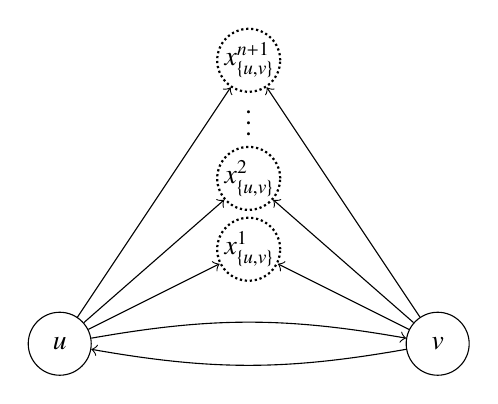
\begin{tikzpicture}[node distance=0.8cm, >=stealth,scale=0.6]

			\tikzset{}

			\node[e4b node] (u) at (0, 0) {$u$};
			\node[e4b node] (v) at (8, 0) {$v$};
			
			% Draw intermediate nodes w
			\node[e4b node,densely dotted, thick] (w1) at (4, 2) {$x_{\{u,v\}}^1$};
			\node[e4b node,densely dotted, thick] (w2) at (4, 3.5) {$x_{\{u,v\}}^2$};
			\node (dots) at (4, 4.85) {$\vdots$};
			\node[e4b node,densely dotted, thick] (wn) at (4, 6) {$x_{\{u,v\}}^{n+1}$};
			
			% Draw edges from u to w's
			\path[e4c path]
			(u) edge[e4c edge] (w1)
			(u) edge[e4c edge] (w2)
			(u) edge[e4c edge] (wn)
			(v) edge[e4c edge] (w1)
			(v) edge[e4c edge] (w2)
			(v) edge[e4c edge] (wn)
			(u) edge[e4c edge, bend left=10] (v)
			(v) edge[e4c edge, bend right=-10] (u)
			;
		\end{tikzpicture}
	\end{center}
	
	Observe that if $\alpha \ge 1/2$,
	a node $v$ can have the value of PageRank less than $c$ in a subgraph $G''$ of $G$
	only if it does not have any incoming edges in $G''$.
	Indeed, if it has at least one incoming edge, say from $u$, then
	$\prm^\alpha_{G''}(v) \ge 1 + \nicefrac{\alpha}{\deg^+_{G''}(u)} \ge c$.
	Thus, the question of the decision variant of \absorbrank\ in the instance $I$ can be equivalently expressed as follows: \emph{Does there exist a subset $S \subseteq V$ with $|S| = k$ such that $\deg^-_{G - E^+(S)}(i) > 0$ for every $i \in S$ (i.e., there is no node in $S$ that has a zero in-degree after the removal of the outgoing edges of nodes in $S\!$)?}
% 
	Let us show that the positive answer to this question for $I$ is equivalent
	to the existence of an indpendent set of size $r$ in $I'$.
	
	First, assume that there is an independence set $R$ of size $r$ in $G'$. We will show that this implies that $S = R \cup V_{new}$, i.e.,
	the subset of the original nodes corresponding to $R$ together with all the new nodes,
	witnesses that $I$ is a yes-instance as well.
	Observe first that $|S| = r+m(n+1) = k$.
	Thus, it remains to show that every node in $S$ has a positive in-degree in the graph $G - E^+(S)$.

	Fix an arbitrary $i \in S$.
	If $i \in V_{new}$, then let $\{u,v\} \in E'$ be an associated edge.
	Since $R$ is an independent set it must be that $u \not \in R$ or $v \not \in R$.
	But this implies that in the graph $G - E^+(S)$,
	node $i$ receives an edge from $u$ or from $v$,
	so it has a positive in-degree.
	If, on the other hand, $i \in R$, then by our assumption that no node has degree of 0 in $G'$,
	we know that there is a $j \in V'$ such that $\{i,j\} \in E'$.
	Since $R$ is an independent set, it holds that $j \not \in R$.
	Thus, $i$ receives an edge from $j$ in the graph $G - E^+(S)$,
	hence it has a positive in-degree.
	This concludes the proof of the forward direction.

	For the reverse direction, assume that there exists a subset $S \subseteq V$ such that $|S| = k$
	and for every $i \in S$ it holds that $\deg^-_{G - E^+(S)}(i) > 0$.
	We will show that this implies the existence of an independent set of size $r$ in $G'$.
	Let us denote by $R$ the set of original nodes belonging in $S\!$, formally, $R := S \setminus V_{new}$.
	Since there are $m(n+1)$ new nodes in total,
	we can show that $R$ has to contain at least $r$ nodes.
	Indeed, $|R| = |S \setminus V_{new}| \ge |S| - m(n+1) = k - m(n+1) =r$.

	We will now prove that $R$ has to be an independent set in $G'$.
	For a contradiction assume that this is not the case, i.e.,
	there exists an edge $\{u,v\} \in E'$ such that $u,v \in R$.
	Observe that there must be a new node $x^i_{\{u,v\}}$, for some $i \in [n+1]$,
	that is selected to $S$.
	Otherwise, if all the new nodes associated with the egde $\{u,v\}$ were not in $S$,
	the size of $S$ would be too small, i.e.,
	$|S| \le |V| - (n+1) = m(n+1) + n - (n+1) = m(n+1) - 1 < k$.
	Since both $u$ and $v$ are in $S$,
	node $x^i_{\{u,v\}}$ has no incoming egdes in $G - E^+(S)$,
	which contradicts our assumption proving that $R$ is indeed an independent set.
	\hfill \qed


\subsection[Proof of Theorem~\ref{thm:polynomial}]{Proof of \cref{thm:polynomial}}

First, we observe
that \absorbrank and \absorbkatz can be computed in polynomial time when applied to bipartite graphs.
If the number of nodes with incoming edges, i.e., $|V_2|$, is at least $k$,
then those rules simply coincide with their \top counterparts. 
Otherwise, if $|V_2| < k$, then both \absorbrank and \absorbkatz
output any subset of nodes of size $k$
as the minimum centrality in such a subset is necessarily $1$.
Thus, in the remainder of the proof let us focus on functional graphs.
Observe that on such graphs, \absorbrank coincides with \absorbkatz,
simply because the two centralities are equivalent when the out-degree of every node is at most $1$.
Therefore, we focus on \absorbrank below.

It holds that if $G = (V,E)$ is a functional graph
and $S \subseteq V$ is an arbitrary subset of nodes,
then in the graph $G - E^+(S)$ each node $i \in S$
is a root of some in-tree,
i.e., a connected functional graph without a cycle.
This means that PageRank of $i$ for $\alpha \rightarrow 1$
is just equal to the number of $i$'s predecessors in this graph.
Hence,
$\prm^{\alpha \rightarrow 1}_G(S) = \min_{i \in S} |\Pred_{G - E^+(S)}(i)|.$
Therefore, we get that
\absorbrank chooses a subset of nodes $S \subseteq V$
that maximizes the minimal number of predecessors of nodes from $S$
in $G - E^+(S)$.
To find such a subset,
given parameters $p,\ell \in \mathbb{N}$ and a functional graph $G = (V,E)$,
we ask whether there is a subset $S \subseteq V$ of size $\ell$,
such that each node $i \in S$ has at least $p$ predecessors in $G - E^+(S)$.
We will denote this decision problem by $\Pi(G,p,\ell).$
Deciding $\Pi(G,p,\ell)$ for all possible values of $p$ (which are upper bounded by $|V|$) and selecting the set $S$ that witnesses that $\Pi(G,p,k)$ is a \emph{yes}-instance for the maximum possible value of $p,$ solves the optimization version of \absorbrank.
  
It holds that $\Pi(G,p,\ell)$ can be solved in polynomial time for in-trees~\citep{perl1981max,frederickson1991optimal}.
We refer to such a procedure as $\texttt{alg-tree}(G,p,\ell)$.
In what follows, we extend $\texttt{alg-tree}(G,p,\ell)$
first to arbitrary connected functional graphs (possibly with a cycle),
and then to all functional graphs (possibly disconnected).


Suppose that $G$ is an arbitrary connected functional graph. 
Observe that $G$ can have at most one cycle
and we can assume that at least one node will be selected form the cycle
(if no node is selected to $S$ from the cycle,
then we can take a selected node that is closest to the cycle,
remove it from $S$,
and instead select a node from the cycle;
such a procedure will not decrease the number of predecessors
in $G - E^+(S\!)$ of any node in $S\!$).
Hence, for each node $v$ in the cycle
we can remove an outgoing edge of this node
and check wether $\Pi(G - E^+(\{v\}), p, \ell)$ is a \emph{yes}-instance
using $\texttt{alg-tree}$.
If this is the case for some node $v$ in the cycle,
we know that $(G,p,\ell)$ is a \emph{yes}-instance as well,
otherwise, it is a \emph{no}-instance.
Let us denote this procedure as \texttt{alg-connected}.


Finally, suppose that $G$ is an arbitrary functional graph.
By $c$ we denote the number of its components and
by $G_1, G_2, \dots, G_c$ the components themselves.
To solve $\Pi(G, p, \ell)$ we us a dynamic programming approach.
Let $A$ be a $c \times \ell$ array.
The values in the first row of $A$
reflect for which numbers $j \in [\ell]$
we can select $j$ nodes in $G_1$
in such a way that each has at least
$p$ predecessors after the removal of their outgoing edges,
i.e,. $A[1,j] = 1$, if
$\Pi(G_1, p, j)$ is a \emph{yes}-instance,
and $A[1,j] = 0$, otherwise.
Since $G_1$ is a connected functional graph, $\Pi(G_1, p, j)$ can be decided using \texttt{alg-connected}.
Then, for each consecutive row $i \in \{2,3,\dots,c\}$,
the values reflect whether 
we can select such $j$ nodes in
$G_1,G_2,\dots,G_i$ jointly.
Thus, $A[i, j] = 1$, if there exists a $j' \in [j]$
such that $A[i-1, j'] = 1$,
and $\Pi(G_i, p, j - j')$ is a \emph{yes}-instance,
i.e., we can select $j'$ nodes in $G_1,G_2,\dots,G_{i-1}$,
and remaining $j - j'$ nodes in $G_i$
(we assume that $\Pi(G', p, 0)$ returns \emph{yes} for every graph $G'$).
Finally, $\Pi(G,s,\ell)$ is a \emph{yes}-instance, if and only if,
$A[c,\ell]=1$.\hfill \qed


\subsection[Proof of Proposition~\ref{prop:axioms_topk}]{Proof of ~\cref{prop:axioms_topk}}
In \cref{fig:toprank_violates} we present a graph that demonstrates that \toprank and \topkatz violate Clique-Entitlement, for $k=3$. The graph consists of 2 components, one of size $2$ that is strongly connected, say $G_1,$ and one of size $4$ that is only weakly connected, say $G_2$.
Under the examined axiom, the nodes from $G_1$ are entitled to $1$ representative in the selected committee. However, the three nodes of maximal PageRank and Katz centrality all belong to $G_2$. As a result, no node from $G_1$ will be selected under \toprank or \topkatz. \hfill \qed

\begin{figure}[t]
	\centering
	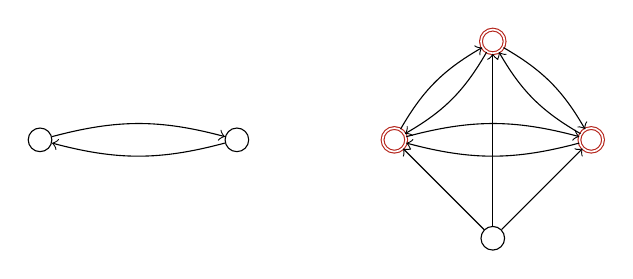
\begin{tikzpicture}[x=5cm,y=5cm] 
		\node[e4c node] (1) at (-0.40, 0.25) {}; 
		\node[e4c node] (2) at (0.10, 0.25) {}; 
		\node[e4c node,selected] (3) at (0.50, 0.25) {}; 
		\node[e4c node,selected] (4) at (0.75, 0.50) {}; 
		\node[e4c node,selected] (5) at (1.00, 0.25) {}; 
		\node[e4c node] (6) at (0.75, 0) {}; 
		
		\path[e4c path]
		(1) edge[e4c edge, bend left=15]  (2)
		(2) edge[e4c edge, bend left=15]  (1)
		(3) edge[e4c edge, bend left=15]  (4)
		(4) edge[e4c edge, bend left=15]  (3)
		(3) edge[e4c edge, bend left=15]  (5)
		(5) edge[e4c edge, bend left=15]  (3)
		(4) edge[e4c edge, bend left=15]  (5)
		(5) edge[e4c edge, bend left=15]  (4)
		(6) edge[e4c edge]  (3)
		(6) edge[e4c edge]  (4)
		(6) edge[e4c edge]  (5)
		;
		
	\end{tikzpicture}
		\caption{An example demonstrating that \toprank and \topkatz violate Clique-Entitlement (\cref{prop:axioms_topk}). Nodes with \textcolor{BrickRed}{red} double lines have the highest PageRank and Katz centrality.}
	\label{fig:toprank_violates}
\end{figure}
%\end{proof}

\subsection[Proof of Theorem~\ref{prop:axioms_absorb}]{Proof of \cref{prop:axioms_absorb}}

Let us start by showing that \absorbkatz violates Clique-Entitlement.
To this end, we will use the Katz recursive formula that is an equivalent definition of Katz centrality~\citep{Kat-1953-KatzCentrality}.
It relates the centrality of a node to the centrality of its direct predecessors as follows:
\[ \katz^{\alpha}_G(v) = \alpha \sum_{(u,v) \in E} \katz^{\alpha}_G(v) + 1 \]
Let us denote an $n$-clique by $K_n$.
Simple calculations based on the above formula
show that
\[
	\katz^{\alpha}_{K_n}(v) = \frac{1}{1-(n-1)\alpha}.
\]
Hence, Katz centrality of a node in a clique is strictly increasing
with the size of the clique for a given $\alpha$.
Moreover, observe that if we remove outgoing edges of a node in an $n$-clique, then Katz centrality of the remaining nodes will be equal to the centrality in $(n-1)$-clique---the existence of this node does not affect the number of walks ending in other nodes.
Thus, if we have a graph in which one third of all nodes form clique $K_n$
and two thirds form clique  $K_{2n}$,
then, for $k < n$, \absorbkatz would select only nodes from the larger clique.
This clearly violates Clique-Entitlement.
	
	\begin{figure}[t]
		\centering
		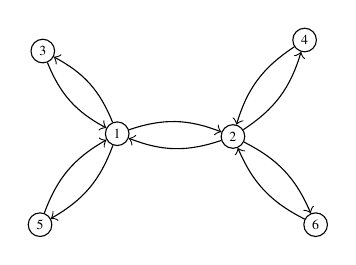
\begin{tikzpicture}[x=3.5cm,y=3.5cm] % change these values to adjust the size of a figure
			\node[e4c node] (1) at (0.28, 1.22) {1}; 
			\node[e4c node] (2) at (0.70, 1.21) {2}; 
			\node[e4c node] (3) at (0.01, 1.52) {3}; 
			\node[e4c node] (4) at (0.96, 1.56) {4}; 
			\node[e4c node] (5) at (0.00, 0.89) {5}; 
			\node[e4c node] (6) at (1.00, 0.89) {6}; 
			
			
			\path[e4c path]
			(3) edge[e4c edge, bend right=20]  (1)
			(1) edge[e4c edge, bend right=20]  (3)
			(1) edge[e4c edge, bend left=20]  (5)
			(5) edge[e4c edge, bend left=20]  (1)
			(1) edge[e4c edge, bend left=20]  (2)
			(2) edge[e4c edge, bend left=20]  (1)
			(4) edge[e4c edge, bend right=20]  (2)
			(2) edge[e4c edge, bend right=20]  (4)
			(2) edge[e4c edge, bend left=20]  (6)
			(6) edge[e4c edge, bend left=20]  (2)
			;
		\end{tikzpicture}
		
		\caption{A component of the graph used in the proof that \absorbrank does not satisfy Component-Entitlement (\cref{prop:axioms_absorb}).} 
		\label{fig:minmaxpr:scc}
	\end{figure}

Now, let us prove that \absorbrank violates Component-Entitlement.
To this end, consider graph $G=(V,E)$ that consists of a clique of 24 nodes and disconnected from that a subgraph identical to that presented in \cref{fig:minmaxpr:scc}.
Let us set $k=15$, i.e., we want to select half of the nodes.
By Component-Entitlement this would mean that we need to select 3 nodes from the structure in \cref{fig:minmaxpr:scc}. However, \absorbrank will select at most 2 from there. Specifically, if we select 2 from the structure and 13 from the clique, we get PageRank 2.98 for each in the structure and 1.83 for each from the clique, resulting in a minimum of 1.83.
On the other hand, say that we select 3 from the structure and 12 from the clique. Then, we get PageRank of 1.90 for each in the clique. If we pick the 2 middle nodes from the structure or 1 middle and a neighbor of it, then we have a PageRank of 1. If we pick 1 middle and 2 non-neighboring (e.g. 1 and 4,6) then the minimum PageRank equals 1.33. If we pick 0 from the middle (e.g. picking 3,5,6) then the minimum PageRank equals 1.78. As a result, \absorbrank will pick at most 2 from the structure, since, adding any node as third, results in lower minimal PageRank than 1.83.
	

In the remainder of the proof,
let us show that \absorbrank satisfies Clique-Entitlement.
To this end, consider arbitrary graph $G = (V,E)$,
in which there exists a strongly connected component $S$
such that $G[S]$ is a clique.
Let $W \subseteq V$ be an arbitrary subset of nodes of size $|W| = k < n$.
Also, let us denote the number of nodes from $S$ in $W$ by $\ell = |W \cap S|$.
We will first prove the following bounds on PageRanks of nodes in $W$
in the graph with outgoing edges of $W$ removed:
\begin{align}
	\label{eq:clique-ent:1}
	\prm^{\alpha \rightarrow 1}_{G - E^+(W)}(i) &= \nicefrac{|S|}{\ell}, \quad \mbox{for every } i \in W \cap S, \mbox{ and} \\
	\label{eq:clique-ent:2}
	\prm^{\alpha \rightarrow 1}_{G - E^+(W)}(j) &\le \nicefrac{(n - |S|)}{(k - \ell)}, \quad \mbox{for some } j \in W \setminus S.
\end{align}
Then, we will show that both formulas imply
that whenever the Clique-Entitlement condition is not satisfied, i.e.,
$\ell < \lfloor k \cdot \nicefrac{|S|}{n} \rfloor$, then
the minimum PageRank of nodes from $W$ in $G - E^+(W)$ can be increased.
Since \absorbrank maximizes this minimum,
this will mean that \absorbrank satisfies Clique-Entitlement.

We note that for every node $v \in V$ with a successor that does not have outgoing edges,
Equation~\eqref{eq:pagerank} is also well defined for $\alpha=1$
(as the probability that the random walk returns to $v$ after visiting it
is strictly less than 1,
the expected number of visits in the walk is finite).
Thus, since we will consider only such nodes,
to simplify our calculations, we will consider PageRank with $\alpha=1$.

To prove Equation~\eqref{eq:clique-ent:1},
we will use PageRank's recursive formula,
which is an equivalent definition of PageRank~\citep{PagBriMotWin-1999-PageRank}.
The formula relates PageRank of a node
with PageRanks of the nodes from which it receives incoming edges as follows
\[
	\prm^\alpha_G(v) = 1 + \alpha \cdot \sum_{(u,v) \in E} \frac{\prm^\alpha_G(u)}{\deg^+(u)}.
\]
Consider an arbitrary unselected node in the clique, i.e., $v \in S \setminus W$.
Since in graph $G - E^+(W)$, node $v$ receives one edge from every other node in $S \setminus W$
and each such node has an out-degree of $|S|-1$,
by PageRank's recursive formula
\[
	\prm^1_{G - E^+(W)}(v) =
	1 + \frac{1}{|S|-1} \cdot \sum_{u \in S \setminus W \setminus \{v\}} \prm^1_{G - E^+(W)}(u).
\]
Now, when we sum this equation side-wise for all $v \in S \setminus W$,
on the right-hand side of the equaiton,
 $\prm^1_{G - E^+(W)}(u)$ for each node $u$
will appear $|S \setminus W| - 1 = |S| - \ell - 1$ times.
Thus,
\[
	\sum_{v \in S \setminus W} \prm^1_{G - E^+(W)}(v) =
	|S| - \ell + 
	\frac{|S| - \ell - 1}{|S|-1} \sum_{u \in S \setminus W} \prm^1_{G - E^+(W)}(u).
\]
Moving the sum to one side and dividing by
$1 - \nicefrac{(|S| - \ell - 1)}{(|S|-1)} = \nicefrac{\ell}{(|S| - 1)}$,
we get
\[
	\sum_{v \in S \setminus W} \prm^\alpha_{G - E^+(W)}(v) =
	(|S| - \ell) \frac{|S| - 1}{\ell}.
\]
% Going with $\alpha$ to the limit of $1$, we clearly obtain
%  \[
% 	\sum_{v \in S \setminus W} \prm^{\alpha \leftarrow 1}_{G - E^+(W)}(v) =
% 	\frac{|S| - 1}{|S| - 1 - |S| + \ell + 1} =
% 	\frac{|S| - 1}{\ell}.
% \]

Then, take an arbitrary node $i \in S \cap W$ and observe that it receives one edge from every node in $S \setminus W$.
Thus,
\[
	\prm^1_{G - E^+(W)}(i) =
	1 + \frac{1}{|S|-1} \cdot \sum_{v \in S \setminus W} \prm^\alpha_{G - E^+(W)}(v) =
	1 + \frac{|S| - \ell}{\ell} =
	\frac{|S|}{\ell}.
\]
Hence, Equation~\eqref{eq:clique-ent:1} indeed holds.

Next, let us prove Inequality~\eqref{eq:clique-ent:2}.
To this end, let us denote by $T$ the set of all predecessors of nodes in $W \setminus S$
that are not selected to $W$ themselves, i.e.,
$T = \{v \in V: \exists_{u \in W} v \in \Pred(u)\} \setminus W$.
Then, let us sum PageRank's recursive formula sidewise,
for all nodes $v \in T$.
We obtain
\[
	\sum_{v \in T} \prm^1_{G - E^+(W)}(v) =
	|T| + 
	\sum_{(u, v) \in E : v \in T} \frac{\prm^1_{G - E^+(W)}(u)}{\deg^+(u)}.
\]
For every $u \in T$,
let $d_w(u)$ be the number of edges that go to nodes in $W$ (possibly $d_w(v)=0$),
while by $d_r(u)$ let us denote the number of its remaining outgoing edges, i.e.,
$d_r(u) + d_w(u) = \deg^+(u)$.
Observe that every node that has an outgoing edge to a node in $T$ must be in $T$ itself.
Thus, the set of edges between nodes in $T$
is exactly the same as the set of all edges counted in $d_r(u)$ for some $u \in T$.
This gives us
\[
	\sum_{v \in T} \prm^1_{G - E^+(W)}(v) =
	|T| + 
	\sum_{u \in T} \left(\frac{d_r(u)}{\deg^+(u)}\prm^1_{G - E^+(W)}(u)\right).
\]
Moving all PageRanks to the left-hand side, we get
\[
	\sum_{v \in T}  \left(\frac{d_w(v)}{\deg^+(v)}\prm^1_{G - E^+(W)}(v)\right) =
	|T|.
\]

Now, let us sum the PageRank's recursive formula for all $j \in W \setminus S$.
We get
\[
	\sum_{v \in (N \setminus S) \cap W} \prm^1_{G - E^+(W)}(v) =
	k - \ell + 
	\sum_{(u, v) \in E : v \in (N \setminus S) \cap W} \frac{\prm^1_{G - E^+(W)}(u)}{\deg^+(u)}.
\]
Observe that the set of all incoming edges to nodes in $W \setminus S$
is exactly the set of edges that are counted in $d_w(u)$ for some $u \in T$.
Thus, we get
\[
	\sum_{v \in (N \setminus S) \cap W} \prm^1_{G - E^+(W)}(v) =
	k - \ell + 
	\sum_{u \in T} \left(\frac{d_w(v)}{\deg^+(v)}\prm^1_{G - E^+(W)}(v)\right) =
	k - \ell + |T| \le
	k - \ell + (n - |S| - (k - \ell)) =
	n - |S|.
\]
Then, Inequality~\eqref{eq:clique-ent:2} follows from the pigeonhole principle.

Next, let us show that if
$\ell \le \lfloor k \cdot \nicefrac{|S|}{n} \rfloor$,
then a node in $W$ with minimum PageRank is in set $V \setminus S$.
To this end, observe that
\[
\frac{|S|}{\ell} \ge \frac{|S|}{\lfloor k \cdot \nicefrac{|S|}{n} \rfloor} \ge \frac{n}{k}.
\]
Multiplying both the nominator and the denominator by $(1 - \nicefrac{|S|}{n})$, we obtain
\[
	\frac{|S|}{\ell} \ge \frac{n(1 - \nicefrac{|S|}{n})}{k (1 - \nicefrac{|S|}{n})} = \frac{n - |S|}{k - k \cdot \nicefrac{|S|}{n}} \ge  \frac{n - |S|}{k - \lfloor k \cdot \nicefrac{|S|}{n} \rfloor} \ge \frac{n - |S|}{k - \ell}.
\]
Thus, by Equation~\eqref{eq:clique-ent:1} and Inequality~\eqref{eq:clique-ent:2},
indeed, if $\ell \le \lfloor k \cdot \nicefrac{|S|}{n} \rfloor$, then
$\min_{i \in W}\prm^1_{G - E^+(W)}(i) \le \frac{n - |S|}{k - \ell}$.
This means, that as long as the inequality is strict, i.e.,
$|S \cap W| < \lfloor k \cdot \nicefrac{|S|}{n} \rfloor$,
the minimum can be increased by removing a node with minimal PageRank from $W$
and adding to $W$ another node from the set $S$.
This means that \absorbrank satisfies Clique-Entitlement.
\hfill \qed

\subsection[Proof of Theorem~\ref{prop:axioms_mes}]{Proof of \cref{prop:axioms_mes}}
Our proof is based on the fact that the Method of Equal Shares
satisfies a property called \emph{priceability} \citep{PetPieSko-2021-EqualSharesPB}.
The property portrays an election as a market
in which the voters who control equal parts of a budget
will jointly pay for candidates.  

Given an election profile $(V, C, \mu)$ and requested committee size $k$,
a price system is a pair $\mathcal{P} = (b , p)$,
where $b \in \mathbb{R}$, $b \ge k$ is an \emph{initial budget}
(where each voter controls an equal part of the budget, i.e., $\nicefrac{b}{n}$)
and $p = (p_i)_{i \in V}$ is a sequence of \emph{payment functions}
where for each $i \in V$ the function
$p_i : C \rightarrow \mathbb{R}_{\ge 0}$
represents how much money voter $i$ spends for each candidate.
We will assume that each candidate costs 1 unit of money.
Then, a committee $W$ is \emph{supported by the price system} $\mathcal{P}$
if the following conditions hold:
\begin{enumerate}
	\item The voters do not pay for candidates they do not support, i.e., $\mu_i(c) = 0$ implies that $p_i(c) = 0$ for every $i \in V$ and $c \in C$.
	\item The sum of payments by $i$ does not exceed their budget, i.e.,
		$\sum_{c \in W} p_i(c) \le \nicefrac{b}{n}$.
	\item Each elected candidate is fully paid, i.e.,
		$\sum_{i \in V} p_i(c) = 1$ for every $c \in W$.
	\item The voters do not pay for unelected candidates,
		i.e., $p_i(c)=0$ for every $i \in V$ and $c \in C \setminus W$.
	\item For each unselected candidate, its supporters do not have enough money to buy it, i.e.,
		$\sum_{i \in V: \mu_i(c) > 0} (\nicefrac{b}{n} - \sum_{c' \in W}p_i(c')) < 1$.
\end{enumerate}

A committee $W$ is \emph{priceable} if there is a price system $\mathcal{P}$ that supports it.
\citet{PetPieSko-2021-EqualSharesPB} observed that MES always outputs a priceable outcome.
We will use this fact to show that it satisfies Subgraph-Entitlement.

Assume otherwise and
take an arbitrary graph $G = (V,E)$, constant $k < n$,
and utility function $\mu_G : V \times V \rightarrow \mathbb{R}_{\ge 0}$
such that $\mu_G(u, v) > 0 \Leftrightarrow u \in Pred(v)$
and there exists a subset $S$
with $G[S]$ being strongly connected
for which $|(S \cup \Succ(S)) \cap W| \le \lfloor k \cdot \nicefrac{|S|}{n} \rfloor - 1$,
where $W$ is an outcome of MES on election $(V, V, \mu_G)$
with committee size $k$.

Since $W$ is priceable, we know that there exists
a price system $\mathcal{P} = (b, p)$ that supports it.
First, let us show that each node $v \in S$
can pay only for nodes in $(S \cup \Succ(S)) \cap W$, i.e.,
$p_v(u) = 0$ for every $v \in S$ and $u \not \in (S \cup \Succ(S)) \cap W$.
Indeed, for $u \not \in S \cup \Succ(S)$, there is no walk from $v$ to $u$,
hence by our assumption on $\mu_G$ and condition 1 of a priceable system,
we get that $p_v(u) = 0$.
Moreover, $p_v(u)=0$ for $u \not \in W$ by condition 4.

Thus, we can show the following lower bound on the money that is unspent by nodes in $S$.
\begin{align}
	\notag
	\frac{|S| \cdot b}{n} - \sum_{v \in S} \sum_{c \in C} p_v(c) &=
	\frac{|S| \cdot b}{n} - \sum_{v \in S} \sum_{c \in (S \cup \Succ(S)) \cap W} p_v(c) \\ &\ge
	\tag{increase the set over which we sum}
	\frac{|S| \cdot b}{n} - \sum_{v \in V} \sum_{c \in (S \cup \Succ(S)) \cap W} p_v(c) \\ &=
	\tag{by condition 3}
	\frac{|S| \cdot b}{n} - |(S \cup \Succ(S)) \cap W| \\ &\ge
	\tag{as $S$ is supposed to witness Subgraph-Entitlement violation}
	\frac{|S| \cdot b}{n} - \left(\left\lfloor k \cdot \frac{|S|}{n} \right\rfloor - 1\right) \\ &\ge
	\tag{since $\lfloor x \rfloor \le x$}
	\frac{|S| \cdot b}{n} - k \cdot \frac{|S|}{n} + 1 \\ &\ge
	\tag{since $b \ge k$}
	1.
\end{align}

Now, let us show that there must exist a node in $S$ that is unselected to $W$.
Assume otherwise, i.e., $S \subseteq W$.
Then, $(S \cup \Succ(S)) \cap W = S \cup (\Succ(S) \cap W)$.
Moreover, since $S$ is witnessing Subgraph-Entitlement violation, we get
\[
	|S| \le |S \cup (\Succ(S) \cap W)| = |(S \cup \Succ(S)) \cap W| \le \lfloor k \cdot \nicefrac{|S|}{n} \rfloor - 1 \le k \cdot \nicefrac{|S|}{n} - 1.
\]
However, this is a contradiction as
this implies that $0 \le \nicefrac{(n-k)}{n} \cdot |S| \le -1$.

Therefore, there is a node $i \in S \setminus W$.
Since $S$ is strongly connected,
by assumption that
$\mu_G(u, v) > 0 \Leftrightarrow u \in Pred(v)$,
it must be that $i$ is supported by all voters in $S$.
On the other hand, as we have shown, these voters have together at least 1 unit of money,
which contradicts condition 5 of a price system.
\hfill \qed

 



\end{document}
